\chapter{Fundamentos. Corriente continua}\label{chap.cc}
	
\setcounter{page}{1}
	
\section{Introducción}
	
La electricidad constituye una forma de energía que está presente en
casi todas las actividades del hombre de una sociedad desarrollada, ya
que gran parte de los aparatos y máquinas que usamos funcionan con
ella. Produce efectos luminosos, mecánicos, caloríficos, químicos,
etc., y se debe a la separación o movimiento de los electrones que
forman los átomos. Las primeras observaciones de la atracción
eléctrica ocurrieron en la antigua Grecia, donde observaron que, al
frotar ámbar, éste atraía pequeños objetos livianos (paja, plumas,
tela...). De hecho, el concepto de fuerza eléctrica tuvo su origen en
experimentos muy sencillos como la frotación de dos cuerpos entre sí,
al ver que cuando se frota una varilla de vidrio o de ámbar con un
trapo o piel, éstas son capaces de desplazar piezas muy ligeras. Así,
apareció la propiedad llamada \textbf{carga eléctrica} que causa este
comportamiento. Además, se observaron dos tipos de acciones,
\textbf{atracción} y \textbf{repulsión}, asociadas, por tanto, a la
existencia de dos tipos de cargas (positiva y negativa). Con esta
premisa, en el siglo XVIII, Benjamin Franklin sugirió que todo objeto
posee una cantidad ``normal'' de electricidad y, cuando dos objetos se
frotan entre sí, parte de la electricidad se transfiere de un cuerpo
al otro.
	
Además, la fuerza que actúa sobre dos cuerpos cargados es proporcional
al producto de las cargas e inversamente proporcional al cuadrado de
la distancia que las separa, teniendo en cuenta que cargas iguales se
repelen y distintas se atraen (ley de Coulomb). El medio en que se
encuentren las cargas va a influir en dicha fuerza, reflejado mediante
la constante de proporcionalidad $k$ (constante de Coulomb):
\begin{equation*}\label{eq.coulomb}
  \Vec{F}=k\cdot\dfrac{Q_1\cdot Q_2}{r^2}\cdot \Vec{u}
\end{equation*}
Esta fuerza es debida a la creación de un campo eléctrico
$\Vec{E}$. Por tanto, se dice que en una región del espacio existe un
\textbf{campo eléctrico} si al situar en ella cargas eléctricas, se
originan fuerzas de tipo electrostático, regidas por la expresión
anterior. De hecho, una carga crea un campo eléctrico en todo el
espacio, y este campo ejerce una fuerza la otra carga. La fuerza es,
por tanto, ejercida por el campo en la posición de la segunda carga,
más que por la propia primera carga que se encuentra a cierta
distancia:
\begin{equation*}
  \Vec{E}=\dfrac{F}{q_0}
\end{equation*}
siendo $q_0$ una carga lo suficientemente pequeña para que su efecto
sobre la distribución de carga sea despreciable. Entonces, el campo
eléctrico es un vector que describe la condición en el espacio creada
por un sistema de cargas puntuales, siendo, por tanto, una función
vectorial de la posición. La fuerza ejercida sobre la carga testigo
$q_0$ en cualquier punto está relacionada con el campo eléctrico por:
\begin{equation*}
  \Vec{F}=q_0\cdot \Vec{E}
\end{equation*}
	
	
\section{Conceptos fundamentales}
	
\subsection{Circuito eléctrico} \label{sec.circuito_electrico}
	
Un \textbf{circuito eléctrico} es un conjunto de componentes
eléctricos combinados de tal forma que crean un camino cerrado por el
que puede circular una corriente eléctrica. %
	%
% \begin{theorem}[Circuito eléctrico]
% Conjunto de elementos combinados de tal forma que existe la
% posibilidad de que se origine una corriente eléctrica.
% \end{theorem}
	%
Hay dos tipos de elementos que se pueden integrar en un circuito
eléctrico:
\begin{itemize}
\item \textbf{Elementos activos.} Dispositivos eléctricos que actúan
  como causas o factores motivantes para la circulación de la
  corriente eléctrica (generadores de tensión o corriente).
\item \textbf{Elementos pasivos.} Componentes eléctricos que toman
  energía de los elementos activos para transformarla en otro tipo de
  energía, o acumularla en forma de campo magnético o eléctrico
  (receptores: resistencias, bobinas y condensadores).
\end{itemize}
	
El \textbf{análisis} (o resolución) de un circuito eléctrico existente
persigue determinar sus condiciones de funcionamiento, es decir,
definir las ecuaciones correspondientes al circuito, así como obtener
los valores de determinadas variables importantes a partir de dichas
ecuaciones. Por contra, el \textbf{diseño} (o síntesis) de un circuito
eléctrico tiene como objetivo definir el circuito eléctrico, es decir,
determinar los componentes necesarios y su interconexión, para obtener
unas condiciones de funcionamiento.
	
Este curso está dedicado al análisis de circuitos eléctricos
\textbf{lineales} de \textbf{parámetros concentrados}.
\begin{itemize}
\item Al considerar que todos los circuitos eléctricos se comportan
  como sistemas lineales, se cumplen las dos condiciones mostradas a
  continuación:
  \begin{enumerate}
  \item $f(x + y) = f(x) + f(y)$: La respuesta $f$ a la suma de dos
    entradas $x$ e $y$ es igual a la suma de la respuesta individual a
    cada una de las entradas.
  \item $f(k \cdot x) = k \cdot f(x)$: La respuesta a una entrada que
    está multiplicada por un factor de escala $k$ es igual a
    multiplicar por este factor a la respuesta a la entrada.
  \end{enumerate}
  Al considerar el circuito como lineal, se simplifica su tratamiento
  de los circuitos, y \textbf{se puede aplicar técnicas de resolución
    de ecuaciones lineales}. Sin embargo, debe recordarse que la
  linealidad es una \textbf{aproximación de la realidad}, que no puede
  aplicarse de manera indiscriminada a cualquier componente y en
  cualquier condición. En particular, los \textbf{dispositivos
    electrónicos} como diodos o transistores tienen un
  \textbf{comportamiento} marcadamente \textbf{no lineal}, de forma
  que los circuitos que los contienen no pueden analizarse
  directamente con las técnicas que aquí se exponen sin realizar
  previamente aproximaciones de su funcionamiento.
\item El análisis de circuitos no toma en consideración las
  propiedades espaciales de los circuitos ni de sus componentes, sino
  que los \textit{confina} a elementos puntuales con un modelo de
  \textbf{parámetros concentrados}. Sin embargo, los circuitos
  eléctricos reales ocupan espacio, las máquinas generadoras y los
  receptores tienen grandes dimensiones, y los cables conductores se
  extienden a lo largo de longitudes variopintas. Por ejemplo, un
  conductor real de 100~m se representa con este modelo de parámetros
  concentrados como un conductor ideal con una resistencia en su punto
  medio. Este tratamiento es una simplificación de las ecuaciones del
  electromagnetismo de Maxwell, y es aplicable únicamente cuando las
  dimensiones del circuito real son inferiores a la longitud de onda
  de la señal que circula por el circuito. Así, a la frecuencia de
  50~Hz (habitual en sistemas eléctricos industriales), la longitud de
  onda de la señal es de 6000~km, mientras que a la frecuencia de
  2.6~GHz (característica de la telefonía 4G), la longitud de onda se
  reduce a 11.5~cm.
\end{itemize}
	
\subsection{Variables}
\subsubsection{Tensión eléctrica}
El \textbf{potencial eléctrico} en un punto, $v(t)$, es la energía
potencial que tiene una carga unitaria en ese punto debida al campo
eléctrico. Dado que la fuerza electrostática $\vec{F}$ (definida con
la ecuación~\eqref{eq.coulomb}) es conservativa, la variación de la
energía potencial $dV$ viene dada por:
\begin{equation*}
  dV=-\Vec{F}\cdot d\vec{l}=-q_0\cdot \Vec{E}\cdot d\vec{l}
\end{equation*}
donde $d\vec{l}$ es el desplazamiento que experimenta la carga debido
al campo eléctrico $\Vec{E}$. La \textbf{tensión} o \textbf{diferencia
  de potencial entre dos puntos}, $u_{AB}(t)$
(Figura~\ref{fig:tension_puntos}), es el trabajo realizado por el
campo eléctrico al desplazar una carga unitaria entre esos puntos:
\begin{equation*}
  u_{AB}(t) = v_A(t) - v_B(t) = \frac{dW_{e}}{dq_0}.
\end{equation*}
\begin{figure}[H]
  \centering
  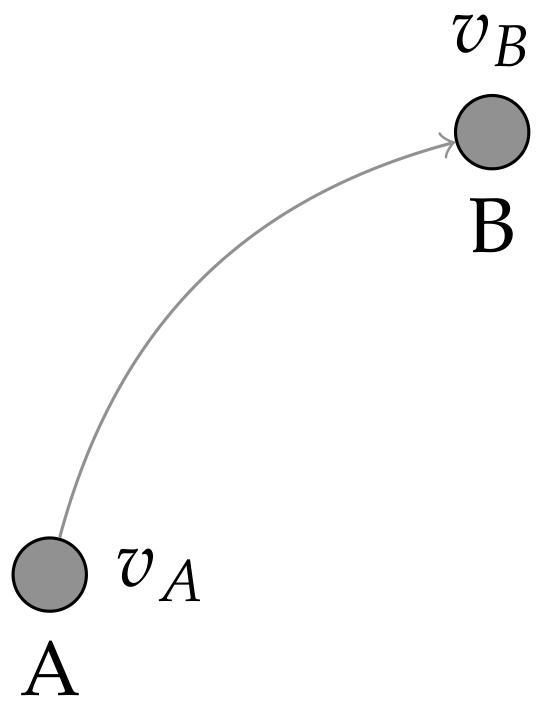
\includegraphics[width=0.2\linewidth]{../figs/tension_puntos.PNG}
  \caption{Diferencia de potencial}
  \label{fig:tension_puntos}
\end{figure}
	
Puesto que el potencial eléctrico es el trabajo electrostático por
unidad de carga, la unidad del SI para $v(t)$ y $u_{AB}(t)$ es el
\textbf{voltio} [V]:
\begin{equation*}
  1\;V=\dfrac{1\;J}{1\;C}.
\end{equation*}
\begin{remark}
  La unidad [V] se escribe en mayúsculas en honor a Alessandro Volta,
  físico y químico italiano del siglo XVIII famoso por la invención y
  desarrollo de la pila eléctrica en 1799.
\end{remark}
Además, el campo eléctrico también es conservativo, por lo que la
diferencia de potencial entre A y B \textbf{no depende de la
  trayectoria} seguida para realizar el desplazamiento, sino
únicamente del potencial existente en cada uno de los puntos
(Figura~\ref{fig:diagrama_tension}). Sin embargo, y pese a que la
trayectoria no es relevante, siempre hay que tener en cuenta el
\textbf{sentido del desplazamiento}
(Figura~\ref{fig:sentido_tension}). Así, si el movimiento se produce
desde B hasta A.
\begin{equation*}
  u_{BA}(t) = v_B(t) - v_A(t) = - u_{AB}(t). 
\end{equation*}
\begin{figure}[H]
  \centering
  \subfloat[Trayectoria]{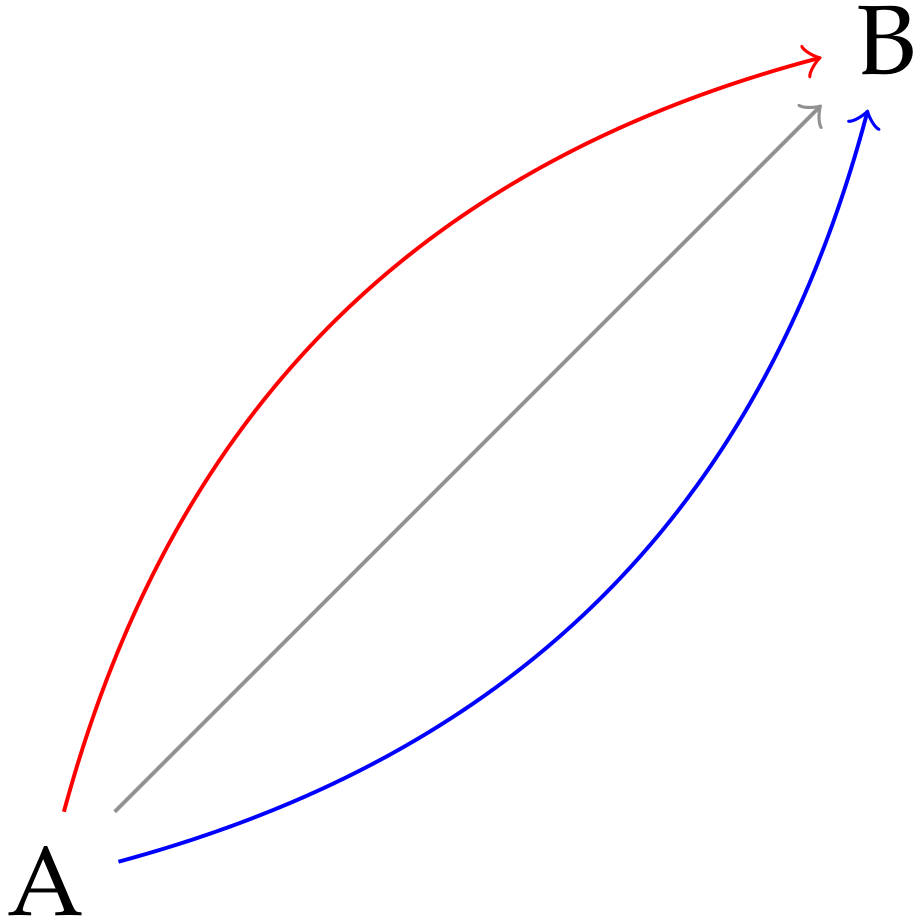
\includegraphics[width=0.25\linewidth]{../figs/diagrama_tension.PNG}\label{fig:diagrama_tension}}\hfil
  \subfloat[Sentido]{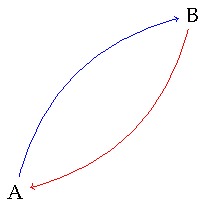
\includegraphics[width=0.25\linewidth]{../figs/sentido_tension.pdf}\label{fig:sentido_tension}}
  \caption{Consideraciones sobre la diferencia de potencial}
\end{figure}
	
	\subsubsection{Corriente eléctrica}
	La \textbf{intensidad de la corriente eléctrica}, $i(t)$, se
        define como la variación de la carga eléctrica $q(t)$ que
        atraviesa la sección transversal de un conductor por unidad de
        tiempo (Figura~\ref{fig:seccion_conductor}).
	\begin{equation*}\label{eq.intensidad}
          i(t)=\dfrac{dq(t)}{dt}
	\end{equation*}
	\begin{figure}[H]
          \centering
          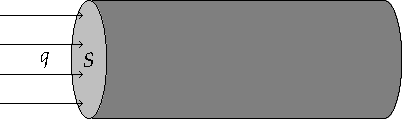
\includegraphics[width=0.45\linewidth]{../figs/seccion_conductor.pdf}
          \caption{Corriente eléctrica}
          \label{fig:seccion_conductor}
	\end{figure}
	
	La corriente eléctrica se produce por el \textbf{movimiento de
          los electrones libres} que fluyen por el conductor, es
        decir, que el \textbf{sentido real} de la intensidad es del
        polo $-$ al polo $+$ del generador (a través del
        conductor). Sin embargo, por razones históricas, el
        \textbf{convenio} que se emplea es justo el opuesto, esto es,
        del polo $+$ al polo $-$. La unidad en el SI de la corriente
        es el \textbf{amperio} [A]:
	\begin{equation*}
          1\,A =\dfrac{1\,C}{1\,s}.
	\end{equation*}
	\begin{remark}
          La unidad [A] se escribe en mayúsculas en honor a
          André-Marie Ampère, matemático y físico francés del siglo
          XVIII-XIX, que inventó el primer telégrafo eléctrico y
          formuló la teoría del electromagnetismo en 1827.
	\end{remark}
	
	Cabe resaltar que el amperio es una unidad muy grande, por lo
        que a menudo se utilizan submúltiplos (mA, $\mu$A...). En
        algunos casos, puede hablarse también de la \textbf{densidad
          de corriente}, definida como el cociente entre la intensidad
        $i(t)$ y la sección transversal del conductor $S$:
	\begin{equation*}
          \delta =\dfrac{i(t)}{S}
	\end{equation*}
	La densidad de corriente se mide en el SI en [A/m$^2$], aunque
        en la industria suele venir determinada en [A/mm$^2$], al ser
        ésta una unidad más manejable.
	
	\subsubsection{Corriente continua y corriente
          alterna} \label{sec.cc-ca} Al estudiar la electricidad, es
        importante destacar que existen dos tipos de corriente: la
        corriente continua y la corriente alterna:
	\begin{itemize}
        \item \textbf{Corriente continua:} La corriente continua es
          aquella que siempre fluye en el mismo sentido (positivo o
          negativo). A su vez, puede ser:
          \begin{itemize}
          \item \textbf{Corriente continua constante:} Su valor
            instantáneo a lo largo del tiempo permanece inalterable
            ($\frac{di(t)}{dt} = 0$, Figura~\ref{fig:continua}). Suele
            estar suministrada por pilas, baterías, dinamos, fuentes
            de alimentación de corriente continua, etc.
            \begin{figure}[H]
              \centering
              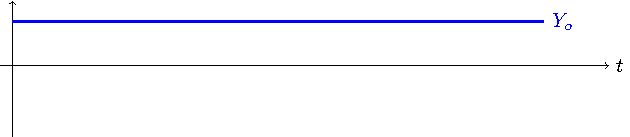
\includegraphics[width=0.75\linewidth]{../figs/continua.pdf}
              \caption{Forma de onda de la corriente continua
                constante}
              \label{fig:continua}
            \end{figure}
          \item \textbf{Corriente continua variable:} Su valor
            instantáneo no es constante a lo largo del tiempo, aunque
            siempre es del mismo signo (negativo o positivo).
          \end{itemize}
        \item \textbf{Corriente alterna:} Aquella corriente que cambia
          de sentido (de positivo a negativo, y viceversa) cada cierto
          tiempo ($\frac{di(t)}{dt} \neq 0$). Se subdivide de nuevo en
          varios tipos:
          \begin{itemize}
          \item \textbf{Corriente alterna sinusoidal:} Los valores
            absolutos instantáneos son sucesivamente proporcionales a
            los valores que toma el seno de 0$^\circ$ a 360$^\circ$
            (Figura~\ref{fig:sinBT1}).
            \begin{figure}[H]
              \centering
              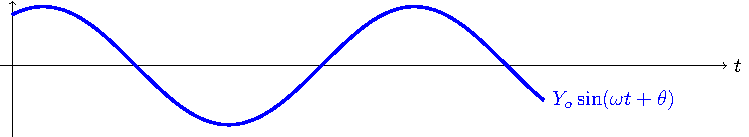
\includegraphics[width=0.75\linewidth]{../figs/sin.pdf}
              \caption{Forma de onda de la corriente alterna senoidal}
              \label{fig:sinBT1}
            \end{figure}
          \item \textbf{Corriente alterna periódica:} Tiene una forma
            de onda que se repite de manera periódica, cambiando de
            sentido, pero no es sucesivamente proporcional a los
            valores que toma el seno de 0$^\circ$ a 360$^\circ$.
          \item \textbf{Corriente alterna aperiódica:} Tiene una forma
            de onda que cambia de sentido pero sin seguir ningún
            periodo.
          \end{itemize}
	\end{itemize}
	Por comodidad, a la corriente continua constante se la conoce
        simplemente como \textit{corriente continua} (CC) y a la
        corriente alterna sinusoidal como \textit{corriente alterna}
        (CA).
	
	
	\subsubsection{Fuerza electromotriz (f.e.m.)}
	En todo circuito eléctrico es necesaria la existencia de al
        menos un elemento activo que suministre energía eléctrica, de
        manera que las cargas permanezcan en movimiento y, por tanto,
        exista corriente eléctrica. La causa capaz de mantener los
        electrones en movimiento en un circuito recibe el nombre de
        \textbf{fuerza electromotriz} (f.e.m.). Los dispositivos
        capaces de proporcionar esta diferencia de potencial
        estacionaria, permitiendo mantener una corriente eléctrica,
        son los \textbf{generadores} (baterías, pilas, dinamos, etc.),
        siendo la f.e.m. ($E$, $e(t)$ o $\epsilon$) la característica
        de éstos.  Por tanto, la fuerza electromotriz representa la
        energía que el generador cede a la unidad de carga
        eléctrica. Al tener la misma naturaleza que la tensión
        eléctrica, también se mide en voltios [V].
	
	\subsubsection{Potencia eléctrica}
	La \textbf{potencia eléctrica} es la variación del trabajo del
        campo eléctrico por unidad de tiempo:
	\begin{equation*}
          p(t)=\frac{dW_{e}}{dt} 
	\end{equation*}
	que puede relacionarse con las variables anteriores:
	\begin{equation*}\label{eq.pvi}
          p(t) = \frac{dW_e}{dq(t)} \cdot \frac{dq(t)}{dt}= u(t)\cdot i(t)
	\end{equation*}
	
	La {unidad} de la potencia eléctrica en el SI es el
        \textbf{vatio} [W]:
	\begin{equation*}
          1\;W = \dfrac{1\;J}{1\;s}= 1\;A\cdot 1\;V.
	\end{equation*}
	\begin{remark}
          La unidad [W] se escribe en mayúsculas en honor a James
          Watt, ingeniero mecánico, inventor y químico escocés de los
          siglos XVIII-XIX, por sus contribuciones al desarrollo de la
          máquina de vapor, fundamental en el desarrollo de la primera
          Revolución Industrial.
	\end{remark}
	
	Para determinar el \textbf{signo de la potencia eléctrica}
        (Figura~\ref{fig:signo_potencia}) hay que tener en
        consideración los signos de las variables de las que depende
        (tensión y corriente):
	\begin{itemize}
        \item Cuando las flechas de ambas variables tienen el
          \textbf{mismo sentido}, la potencia eléctrica es
          \textbf{positiva} ($P>0$)
        \item Cuando las flechas tienen \textbf{sentidos opuestos}, la
          potencia eléctrica es \textbf{negativa} ($P<0$)
	\end{itemize}
	\begin{figure}[H]
          \centering
          \subfloat[$P>0$]{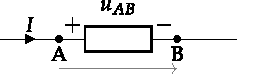
\includegraphics[width=0.3\linewidth]{../figs/signo_potencia1.pdf}}\hfil
          \subfloat[$P<0$]{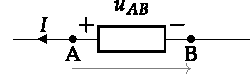
\includegraphics[width=0.3\linewidth]{../figs/signo_potencia2.pdf}}
          \caption{Convenio de signos para la potencia}
          \label{fig:signo_potencia}
	\end{figure}
	En la práctica, no es conveniente trabajar con potencias
        negativas, por lo que es habitual interpretar este resultado
        como potencia absorbida y potencia generada/entregada
        (Figura~\ref{fig:receptor_generador}):
	\begin{itemize}
        \item Un circuito o elemento es un \textbf{receptor} (absorbe
          potencia) cuando la corriente \emph{entra} por el terminal
          de mayor potencial
        \item Un circuito o elemento es un \textbf{generador} (entrega
          potencia) cuando la corriente \emph{sale} por el terminal de
          mayor potencial
	\end{itemize}
	\begin{figure}[H]
          \centering
          \subfloat[Receptor]{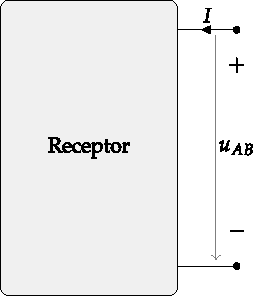
\includegraphics[width=0.25\linewidth]{../figs/receptor_generador1.pdf}}\hfil
          \subfloat[Generador]{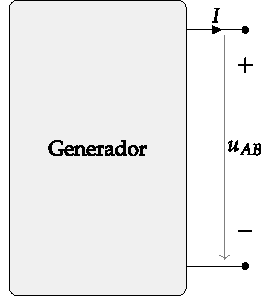
\includegraphics[width=0.25\linewidth]{../figs/receptor_generador2.pdf}}
          \caption{Convenio de signos para la potencia}
          \label{fig:receptor_generador}
	\end{figure}
	
	\begin{remark}
          Téngase en cuenta, que por el principio de conservación de
          la energía, la potencia generada y la potencia consumida en
          un circuito deben ser iguales.
	\end{remark}
	
	\subsubsection{Energía y potencia}
	
	La \textbf{energía} $W$ es una magnitud física asociada con la
        capacidad que tienen los cuerpos para realizar un trabajo
        (emitir luz, generar calor, etc.). Puede manifestarse de
        distintas formas: gravitatoria, cinética, química, eléctrica,
        magnética, nuclear, radiante, etc., existiendo la posibilidad
        de transformar unos tipos de energía en otros, pero respetando
        siempre el principio de conservación de la energía. En el SI,
        la energía (del tipo que sea) se mide en julios [J]. El julio
        se define como el trabajo realizado por una fuerza $F$ de 1
        Newton [N] cuando provoca un desplazamiento $d$ de 1 metro
        [m]. Por tanto, una forma de definir la energía es:
	\begin{equation*}
          W=F\cdot d 
	\end{equation*}
	\begin{remark}
          La unidad [J] se escribe en mayúsculas en honor a James
          Prescott Joule, físico e investigador inglés del siglo XIX,
          considerado como uno de los físicos más notables de su
          época.
	\end{remark}
	
	Dado que la potencia $P$ se define como la cantidad de trabajo
        realizado (es decir, la energía $W$) por unidad de tiempo $t$
        ($P=\frac{W}{t}$), también se puede definir la energía como:
	\begin{equation*}\label{eq.Ept}
          W=P\cdot t
	\end{equation*}
	Por tanto, otra unidad muy utilizada para medir energía es el
        vatio-hora [Wh], aunque ésta \textbf{\emph{no}} es la aceptada
        en el SI. Esta unidad representa el trabajo realizado por una
        máquina de potencia 1 W durante un tiempo de 1 hora. El Wh se
        utiliza comúnmente para medir la \textbf{energía eléctrica}.
	
	\vspace{4mm}
	\begin{example}
          \textbf{¿Cuál es la equivalencia entre un kWh y un J?}
          \begin{equation*}
            1 kWh = 1 kW \cdot 1 h = 1000 W \cdot 3600 s = 3.6 MJ 
          \end{equation*}
	\end{example}
	
	\section{Leyes básicas}
	
	\subsection{Ley de Ohm}
	
	La ley de Ohm, postulada por el físico alemán Georg Ohm
        (1789--1854), es una ley que establece la relación entre la
        tensión y la intensidad de la corriente eléctrica, de acuerdo
        a la expresión:
	\begin{equation}
          \boxed{ U=R\cdot I}
	\end{equation}
        donde $R$ es la resistencia que opone el material al paso de
        la corriente eléctrica (se profundiza más en el concepto de
        \textbf{resistencia} en la Sección~\ref{sec.resistencia}).
	
	\subsection{Leyes de Kirchhoff}
	
	Existen una serie de definiciones previas que es necesario
        conocer para el análisis y la teoría de circuitos eléctricos:
	\begin{itemize}
        \item \textbf{Nudo:} unión de \textbf{3} o más conductores
        \item \textbf{Rama:} elementos conectados entre dos nudos
          consecutivos
        \item \textbf{Lazo:} conjunto de ramas que forman un camino
          cerrado
        \item \textbf{Malla:} lazo que no contiene ningún otro en su
          interior
	\end{itemize}

	\begin{example}\label{ej.1-3}
          \textbf{Determinar el número de nudos, ramas, lazos y mallas
            del circuito de la Figura~\ref{fig:mallas}.}
          \begin{figure}[H]
            \centering
            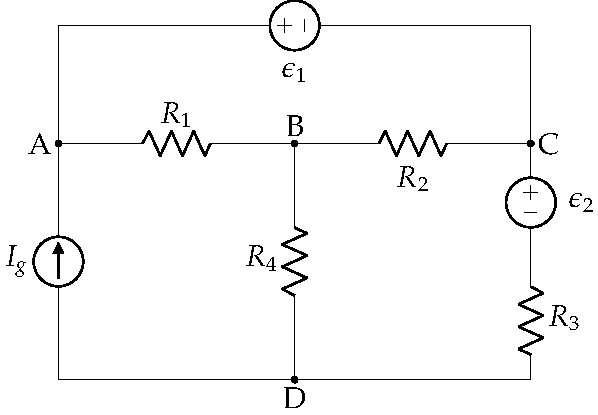
\includegraphics[width=0.5\linewidth]{../figs/mallas.pdf}
            \caption{Ejemplo~\ref{ej.1-3}}
            \label{fig:mallas}
          \end{figure}
		
          Nudos: 4 (A, B, C, D)
		
          Ramas: 6 (AB, AC, AD, BC, BD, DC)
		
          Lazos: 7 (ABDA, BCDB, ACBA, ABCDA, ACBDA, BDCAB, ACDA)
		
          Mallas: 3 (ABDA, BCDB, ACBA)
	\end{example}
	
	
	Aún era un estudiante cuando en 1845 Gustav Robert Kirchhoff,
        a la edad de 21 años, realizó la primera de sus grandes
        aportaciones a la física, formulando las ahora denominadas
        \textbf{leyes de Kirchhoff}, ecuaciones básicas de los
        circuitos eléctricos.
	
	\begin{itemize}
        \item \textbf{Primera ley de Kirchhoff}. Esta ley es el
          resultado directo del \textbf{principio de conservación de
            la carga} aplicado a los circuitos eléctricos. Se conoce
          como primera ley de Kirchhoff (1LK) o ley de Kirchhoff de
          las corrientes (LKC), y dice que la suma algebráica de las
          intensidades de corriente que concurren en un nudo es
          cero. Esto es igual a decir que la suma de las corrientes
          que llegan a un nudo es igual a la suma de las que salen:
          \begin{equation}
            \boxed{\sum_{j=1}^n i_j(t)=0}
          \end{equation}
          Así, en la Figura~\ref{fig:LKC_FM} se cumple que:
          \begin{equation*}
            i_1(t) - i_2(t) + i_3(t) - i_4(t) + i_5(t) = 0
          \end{equation*}
		
		\begin{figure}[H]
                  \centering
                  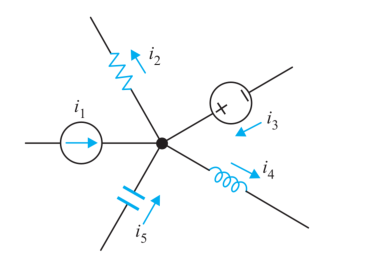
\includegraphics[width=0.35\linewidth]{../figs/LKC_FM.pdf}
                  \caption{Primera ley de Kirchhoff}
                  \label{fig:LKC_FM}
		\end{figure}
              \item \textbf{Segunda ley de Kirchhoff.} Esta ley es
                consecuencia del \textbf{principio de conservación de
                  la energía} aplicado a los circuitos eléctricos. Se
                le denomina segunda ley de Kirchhoff (2LK) o ley de
                Kirchhoff de los voltajes (LKV), y dice que la suma
                (con signo) de las tensiones a lo largo de un circuito
                cerrado es cero. Esto quiere decir que la energía
                producida por un generador es consumida por los
                receptores del circuito para producir algún tipo
                trabajo (mecánico, químico, etc.) o calor:
		\begin{equation}
                  \boxed{\sum_{i=1}^m u_i(t)=0}
		\end{equation}
		Así, en el circuito de la Figura~\ref{fig:LKV_FM}, se
                cumple que:
		\begin{equation*}
                  u_3(t) + u_4 (t) - u_5 (t) - u_1 (t) - u_2 (t)  = 0 
		\end{equation*}
		\begin{figure}[H]
                  \centering
                  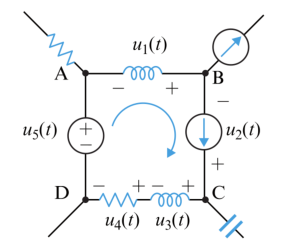
\includegraphics[width=0.35\linewidth]{../figs/LKV_FM.pdf}
                  \caption{Segunda ley de Kirchhoff}
                  \label{fig:LKV_FM}
		\end{figure}
              \end{itemize}
	

	\section{Elementos de los circuitos}
	Como ya se mencionó en la
        Sección~\ref{sec.circuito_electrico}, en un circuito eléctrico
        existen dos tipos de elementos: los elementos pasivos y los
        activos.
	
	\subsection{Elementos pasivos}
	
	En general, en teoría de circuitos se emplean tres tipos de
        elementos pasivos: resistencias, bobinas y condensadores. Se
        dice que un receptor es cualquier dispositivo capaz de
        transformar la energía eléctrica en otra forma de energía (que
        no sea solo calor); así, un ejemplo de receptor es un motor
        eléctrico (transforma parte de la energía eléctrica en
        mecánica).
	
	\subsubsection{Resistencia} \label{sec.resistencia} En el
        siglo XIX, Georg Simon Ohm descubrió la ley que lleva su
        nombre (\textbf{ley de Ohm}). Dicha ley obtiene que, \textit{a
          temperatura constante}, la relación existente entre la
        diferencia de potencial entre los bornes de un conductor y la
        intensidad de corriente que circula por él es una constante,
        denominada \textbf{resistencia eléctrica}:
	\begin{equation*}
          \boxed{u(t)=R\cdot i(t)}
	\end{equation*}
	Por tanto, la resistencia eléctrica representa la mayor o
        menor dificultad que ofrecen los diferentes materiales para
        ser recorridos por una corriente eléctrica. Su valor se mide
        en ohmios [$\Omega$]. El criterio de signos utilizado
        considerar que la tensión es positiva en el terminal por el
        que entra la corriente, esto es, las flechas de tensión y
        corriente tienen el mismo sentido
        (Figura~\ref{fig:resistencia}).
	\begin{figure}[H]
          \centering \subfloat[Referencia mediante
          signo]{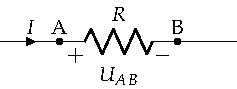
\includegraphics{../figs/Resistencia.pdf}}\hfil
          \subfloat[Referencia mediante
          flecha]{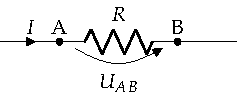
\includegraphics{../figs/Resistencia_Flecha.pdf}}
          \caption{Criterio de signos en una resistencia}
          \label{fig:resistencia}
	\end{figure}
	
	La magnitud que determina si un material es mejor o peor
        conductor se denomina \textbf{resistividad} ($\rho$), medida
        en [$\Omega\cdot$m] en el SI, aunque en las aplicaciones
        prácticas se suele utilizar el [$\Omega\cdot$m$^2/m$]. La
        resistividad de un material permanece constante si no varía la
        temperatura (suele expresarse a 20$^\circ$C). Para conductores
        homogéneos, de sección constante y pequeña comparada con su
        longitud, la resistencia $R$ que ofrece al paso de la
        corriente se puede determinar a partir de:
	\begin{equation*}\label{eq.resistencia_rho}
          R=\rho\cdot \dfrac{l}{S}
	\end{equation*}
	siendo $l$ la longitud del conductor y $S$ el área de la
        sección transversal del mismo. Cabe destacar, por su
        importancia en la industria, la resistividad del cobre
        ($\rho_{Cu}=1/58\;\Omega \cdot$mm$^2/$m) y la del aluminio
        ($\rho_{Al}=1/36\;\Omega \cdot$mm$^2/$m).
	
	\vspace{4mm}
	\begin{example}
          \textbf{Calcular la resistencia de un conductor de cobre que tiene una longitud $l=10$~m y una sección $S=2$~mm$^2$.}\\
          Aplicando la expresión anterior:
          \begin{equation*}
            R=\rho\cdot \dfrac{l}{S}=(1/58)\cdot \dfrac{10}{2}=0.086\;\Omega
          \end{equation*}
	\end{example}
	
	Para temperaturas distintas de 20$^\circ$C, siempre que la
        temperatura final $T_f$ esté en torno a los 250$^\circ$, la
        resistividad y, por tanto, la resistencia pueden determinarse
        a partir de las siguientes expresiones:
	\begin{equation*}
          \rho_f=\rho_{20}\cdot (1+\alpha\cdot (T_f-20)); \qquad
          R_f=R_{20}\cdot (1+\alpha\cdot (T_f-20))
	\end{equation*}
	donde $\rho_f$ y $R_f$ son la resistividad y la resistencia a
        la temperatura $T_f$ (respectivamente), $\rho_{20}$ y $R_{20}$
        son la resistividad y la resistencia a 20$^\circ$C
        (respectivamente) y $\alpha$ es el coeficiente de temperatura.
	
	La inversa de la resistencia se denomina
        \textbf{conductancia}, $G$, y se mide en el SI en
        \textbf{Siemens} [S]. Al ser lo opuesto de la resistencia,
        representa la facilidad de los conductores al paso de la
        corriente eléctrica:
	\begin{equation}
          \boxed{G=\dfrac{1}{R}}
	\end{equation}
	\begin{remark}
          La unidad [S] se escribe en mayúsculas en honor a Ernst
          Werner M. von Siemens, inventor alemán del siglo XIX,
          pionero de la electrotecnia y fundador de la actual empresa
          Siemens.
	\end{remark}
	Asimismo, a la inversa de la resistividad se le denomina
        \textbf{conductividad} ($\gamma$), definida como la facilidad
        que ofrecen los materiales al paso de la corriente eléctrica,
        por unidad de longitud y sección:
	\begin{equation*}
          \gamma=\dfrac{1}{\rho}
	\end{equation*}
	
	El desplazamiento de cargas a través de los conductores
        produce interacciones y choques entre ellas que, a su vez, dan
        origen a un calentamiento del conductor. El físico británico
        James Prescott Joule, en 1841, fue quién cuantificó el valor
        del calor que se produce en un conductor por el paso de la
        corriente y enunció la ley que lleva su nombre (\textbf{ley de
          Joule}): toda la energía que absorbe un conductor homogéneo
        por el que circula una corriente eléctrica y en el que no
        existen f.e.m., se transforma íntegramente en calor. Por
        tanto, la energía ``perdida'' en forma de calor:
	\begin{equation*}
          W=P\cdot t=U\cdot I\cdot t=R\cdot I^2\cdot t
	\end{equation*}
	cuyo resultado viene expresado en [J]. Sin embargo, una unidad
        muy utilizada para medir el calor es la \textbf{caloría}
        [cal], cuya equivalencia con el [J] es:
	\begin{equation*}
          1\;J=0.24\;cal
	\end{equation*}
	En general, se dirá que una resistencia disipa energía
        eléctrica produciendo calor, siendo la potencia disipada:
	\begin{equation*}
          p(t)=R\cdot i^{2}(t)
	\end{equation*}
	
	El concepto de resistencia se utiliza también para definir dos
        términos muy comunes en teoría de circuitos:
	\begin{itemize}
        \item \textbf{Cortocircuito:} Conductor ideal que se une entre
          dos puntos, haciendo de este modo que su resistencia sea
          $R=0\;\Omega$. El cortocircuito puede llevar cualquier
          corriente, cuyo valor depende del resto del circuito, pero
          la tensión entre sus terminales (por la ley de Ohm) es de
          $u_{AB}(t)=0$~V (Figura~\ref{fig:cortocircuito}).
        \item \textbf{Circuito abierto:} Representa una ruptura del
          circuito en ese punto, por lo que no puede circular
          corriente ($i(t)=0$). Se puede considerar como un circuito
          con resistencia infinita ($R\rightarrow\infty$) y que puede
          tener cualquier tensión, que depende del resto de la red
          (Figura~\ref{fig:c_abierto}).
	\end{itemize}
	\begin{figure}[H]
          \centering
          \subfloat[Cortocircuito]{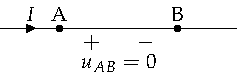
\includegraphics[width=0.25\linewidth]{../figs/cortocircuito.pdf}\label{fig:cortocircuito}}\hfil
          \subfloat[Circuito
          abierto]{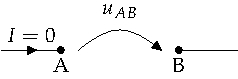
\includegraphics[width=0.25\linewidth]{../figs/CircuitoAbierto.pdf}\label{fig:c_abierto}}
          \caption{Cortocircuito y circuito abierto}
		
	\end{figure}
	
	\subsubsection{Bobina}\label{sec.bobina}
	
	Una \textbf{bobina} es un conductor arrollado, con $N$
        vueltas, alrededor de un núcleo (generalmente, de material
        ferromagnético). La tensión en bornes de la bobina es
        directamente proporcional a la variación de la corriente
        respecto al tiempo, con un factor de proporcionalidad $L$
        conocido como \textbf{inductancia} o coeficiente de
        autoinducción, medido en \textbf{henrios} [H]
        (Figura~\ref{fig:bobina}):
	\begin{equation}\label{eq.u_L}
          \boxed{u(t)=L\cdot\frac{di(t)}{dt}}\,
	\end{equation}
	por lo que, en circuitos de corriente continua, una bobina se
        comporta como un \textbf{cortocircuito}:
	\begin{equation*}
          \dfrac{di(t)}{dt} = 0 \rightarrow u = 0
	\end{equation*}
	\begin{remark}
          La unidad [H] se escribe en mayúsculas en honor a Joseph
          Henry, físico estadounidense del siglo XIX conocido por su
          trabajo acerca del electromagnetismo, electroimanes y relés.
	\end{remark}
	\begin{figure}[H]
          \centering
          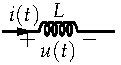
\includegraphics[width=0.15\linewidth]{../figs/Bobina.pdf}
          \caption{Tensión y corriente en una bobina}
          \label{fig:bobina}
	\end{figure}
	
	La relación inversa de la expresión~\eqref{eq.u_L} se puede
        obtener por integración entre un tiempo inicial $t_i$ y un
        tiempo final $t_f$, resultando:
	\begin{equation*}
          \int_{t_i}^{t_f} \dfrac{di(t)}{dt}dt=\dfrac{1}{L}\int_{t_i}^{t_f}u(t)\cdot dt \rightarrow i(t_f)-i(t_i)=\dfrac{1}{L}\cdot\int_{t_i}^{t_f} u(t)\cdot dt\,
	\end{equation*}
	\begin{equation}
          \boxed{i(t_f)=i(t_i)+\dfrac{1}{L}\cdot\int_{t_i}^{t_f} u(t)\cdot dt}
	\end{equation}
	Se observa que la bobina tiene un efecto de ``memoria'', ya
        que la corriente en un tiempo $t_f$ no depende solamente de la
        entrada $i(t)$ en ese momento, sino también del valor inicial
        de la entrada. Además, para establecer un flujo en una bobina,
        es necesario una energía de entrada, que queda almacenada
        después en forma de \textbf{campo magnético}. La potencia
        ``absorbida'' por la bobina será:
	\begin{equation*}
          p(t)=u(t)\cdot i(t)=L\cdot i(t)\cdot\dfrac{di(t)}{dt}
	\end{equation*}
	y la energía almacenada $w(t)$ en un periodo de tiempo entre
        $t_i$ y $t_f$ valdrá:
	\begin{equation*}
          w(t)=\int_{t_i}^{t_f}v(t)\cdot i(t)\cdot dt=\int_{t_i}^{t_f}L\cdot\dfrac{di(t)}{dt}\cdot i(t)\cdot dt=\dfrac{1}{2}\cdot L\cdot [i(t_f)-i(t_i)]^2
	\end{equation*}
	\begin{equation}
          \boxed{w(t)=\dfrac{1}{2}\cdot L\cdot [i(t_f)-i(t_i)]^2}
	\end{equation}
	
	\begin{remark}
          Para entender el concepto de inductancia, es necesario
          recordar algunos principios del electromagnetismo.
          \begin{itemize}
          \item \textbf{Ley de Ampère.} Es la ley fundamental que
            relaciona corrientes eléctricas y campos magnéticos. Su
            versión más simple dice que el producto de $N$ veces una
            corriente $i$ da lugar a una intensidad de campo magnético
            $H$ proporcional a la longitud magnética media de las
            líneas de dicho campo $l$:
            \begin{equation*}
              \label{eq.ampere_mod}
              H\cdot l=N\cdot i
            \end{equation*}
          \item \textbf{Densidad de flujo magnético.} La intensidad de
            campo $H$ origina, allá donde exista, una densidad de
            flujo $B$, cuyo valor es:
            \begin{equation*}\label{eq.B}
              B=\mu\cdot H,
            \end{equation*}
            siendo $\mu$ la permeabilidad del material.
          \item \textbf{Flujo magnético.} Un campo magnético $B$
            (constante en magnitud y dirección) que atraviesa un área
            $S$, formando un ángulo $\theta$ con ésta, crea un flujo
            magnético que se puede calcular como:
            \begin{equation*}\label{eq.flujo1}
              \phi=B\cdot S\cdot \cos (\theta)
            \end{equation*}
          \item \textbf{Ley de Lenz-Faraday.} Un flujo magnético
            variable en el tiempo induce una fuerza electro-motriz
            (fem, $e$) que es igual en magnitud a la variación por
            unidad de tiempo del flujo inducido en el circuito. Esta
            fem inducida tiene un sentido tal que sus efectos tienden
            a oponerse a las causas que lo producen, por lo que:
            \begin{equation*}\label{eq.lenz-faraday}
              e=-\dfrac{d\phi(t)}{dt}.
            \end{equation*}
          \end{itemize}
          A partir de esto, y con la ecuación~\eqref{eq.u_L}, es
          sencillo concluir que, cuando un circuito está formado
          únicamente por una bobina alimentada con una intensidad
          variable (es decir, corriente alterna) el flujo magnético
          también cambia y, por tanto, se induce una $fem$:
          \begin{equation*}
            e=\dfrac{d\phi(t)}{dt}=L\cdot \dfrac{di(t)}{dt} 
          \end{equation*}
          es decir, la $fem$ inducida es proporcional a la variación
          con el tiempo de la intensidad de corriente. Considerando
          esta expresión y despejando el valor de $L$, se tiene que:
          \begin{equation*}
            L= \dfrac{d\phi(t)}{\cancel{dt}}\cdot\dfrac{\cancel{dt}}{di(t)}=\dfrac{d\phi(t)}{di(t)}
          \end{equation*}
          por lo que la inductancia $L$ expresa la relación entre el
          cambio de flujo y el cambio de corriente.
	\end{remark}
	
	
	\subsubsection{Condensador}\label{sec.condensador}
	
	Un sistema de dos placas metálicas separadas por una capa
        dieléctrica constituye un \textbf{condensador}. Al aplicar
        tensión, produciendo una \textbf{separación de cargas
          opuestas} que se \textbf{acumulan} en cada placa (una de las
        placas queda con la carga $+Q$ y la otra con $-Q$). Del mismo
        modo que un elemento resistivo se distingue por el valor de su
        resistencia $R$, y una bobina por el valor de su inductancia
        $L$, un condensador se caracteriza por su \textbf{capacidad}
        $C$, que es la aptitud que tiene para acumular carga
        eléctrica. Así, la capacidad es la relación entre la carga
        $q(t)$ acumulada y la diferencia de potencial aplicada entre
        ellas $u(t)$, siendo:
	\begin{equation}\label{eq.cqu}
          \boxed{C=\dfrac{q(t)}{u(t)}}
	\end{equation}
	La unidad en el SI de la capacidad es el faradio [F]. Se trata
        de una unidad tremendamente grande, por lo que en la práctica
        se utilizan submúltiplos (mF, $\mu$F, pF...).
	\begin{remark}
          La unidad [F] se escribe en mayúsculas en honor a Michael
          Faraday, científico británico de los siglos XVIII-XIX que
          estudió el electromagnetismo y la electroquímica.
	\end{remark}
	
	Durante la carga del condensador, se produce una corriente
        eléctrica entre las dos placas (Figura~\ref{fig:condensador}):
	\begin{equation}\label{eq.icu}
          i(t)=\dfrac{dq(t)}{dt}\stackrel{\eqref{eq.cqu}}{=}\dfrac{d(C\cdot u(t))}{dt}=C\cdot \dfrac{du(t)}{dt} \Rightarrow \boxed{i(t)=C\cdot \dfrac{du(t)}{dt}}
	\end{equation}
	por lo que, en circuitos de corriente continua, un condensador
        se comporta como un \textbf{circuito abierto}.
	\begin{equation*}
          \frac{du(t)}{dt} = 0 \rightarrow i = 0
	\end{equation*}
	\begin{figure}[H]
          \centering
          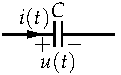
\includegraphics[width=0.15\linewidth]{../figs/Condensador.pdf}
          \caption{Tensión y corriente en un condensador}
          \label{fig:condensador}
	\end{figure}
	
	La relación inversa de la expresión~\eqref{eq.icu} se puede
        obtener por integración entre un tiempo inicial $t_i$ y un
        tiempo final $t_f$, resultando:
	\begin{equation*}
          \int_{t_i}^{t_f} \dfrac{du(t)}{dt}dt=\dfrac{1}{C}\int_{t_i}^{t_f}i(t)\cdot dt \rightarrow u(t_f)-u(t_i)=\dfrac{1}{C}\cdot\int_{t_i}^{t_f} i(t)\cdot dt
	\end{equation*}
	\begin{equation}\label{eq.u_C}
          \boxed{u(t_f)=u(t_i)+\dfrac{1}{C}\cdot\int_{t_i}^{t_f} i(t)\cdot dt}
	\end{equation}
	Se observa que el condensador también tiene un efecto de
        ``memoria'', ya que la tensión en un tiempo $t_f$ no depende
        solamente de la entrada $u(t)$ en ese momento, sino también
        del valor inicial.
	
	Al aplicar tensión a un condensador se produce una separación
        de cargas entre ambas placas, lo que produce un \textbf{campo
          eléctrico}, quedando almacenada una energía de este tipo. La
        potencia ``absorbida'' por el condensador será:
	\begin{equation*}
          p(t)=u(t)\cdot i(t)=C\cdot u(t)\cdot\dfrac{du(t)}{dt}
	\end{equation*}
	y la energía almacenada $w(t)$ en un periodo de tiempo entre
        $t_i$ y $t_f$ valdrá:
	\begin{equation*}
          w(t)=\int_{t_i}^{t_f}v(t)\cdot i(t)\cdot dt=\int_{t_i}^{t_f}C\cdot\dfrac{du(t)}{dt}\cdot u(t)\cdot dt=\dfrac{1}{2}\cdot C\cdot [u(t_f)-u(t_i)]^2
	\end{equation*}
	\begin{equation}
          \boxed{w(t)=\dfrac{1}{2}\cdot C\cdot [u(t_f)-u(t_i)]^2}
	\end{equation}

        \subsection{Elementos activos}\label{sec.elementos_activos}
	
	\subsubsection{Generadores de tensión}
	Un \textbf{generador de tensión} es un dispositivo físico,
        caracterizado por una fuerza electromotriz $\epsilon$ que
        proporciona una diferencia de potencial $U$ entre sus bornes
        de salida. Por tanto, \textbf{impone la tensión} a su salida,
        mientras que \emph{la corriente depende del circuito}
        (Figura~\ref{fig:fuentetension}).
	\begin{itemize}
        \item Un \textbf{generador ideal} es aquel que \textbf{no
            tiene pérdidas}, de tal forma que la diferencia de
          potencial entre sus bornes toma siempre el mismo valor que
          su f.e.m. ($u_{AB}=\epsilon_g$). 
        \item Un \textbf{generador real} es aquel que \textbf{tiene
            pérdidas}, caracterizadas mediante una resistencia
          interna, en \textbf{serie}, $R_{\epsilon_g}$. Al circular
          una corriente por dicha resistencia, se consume en ella una
          potencia que no puede ser entregada por el generador. Las
          pérdidas internas son la causa de que la diferencia de
          potencial entre sus bornes sea inferior a la
          f.e.m. ($u_{AB}<\epsilon_g$). Con esto, la potencia generada
          será $P_g=\epsilon_g\cdot I$, la potencia disipada en la
          resistencia interna $P_p=R_{\epsilon_g}\cdot I^2$ y la
          potencia útil $P_u=U_{AB}\cdot I$ y, dado que tiene que
          cumplirse el principio de conservación de la energía:
          \begin{equation}
            P_g=P_u+P_p\rightarrow \boxed{ \epsilon_g=U_{AB}+ R_{\epsilon_g}\cdot I}
          \end{equation}
	\end{itemize}
	\begin{figure}[H]
          \centering
          \subfloat[Ideal]{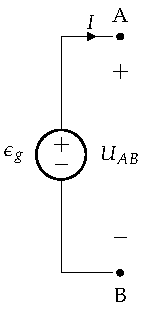
\includegraphics[height=3.5cm]{../figs/FuenteTensionIdealDC.pdf}}\hfil
          \subfloat[Real]{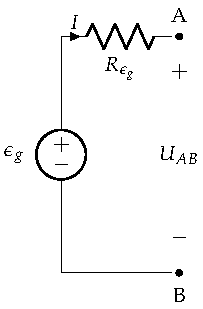
\includegraphics[height=3.5cm]{../figs/FuenteTensionRealDC.pdf}}
          \caption{Generador de tensión}
          \label{fig:fuentetension}
	\end{figure}
	
	\subsubsection{Generadores de corriente}
	Un \textbf{generador de corriente} es un dispositivo físico,
        caracterizado por una intensidad $I_g$ que proporciona una
        corriente $I$. Por tanto, \textbf{impone la corriente} a su
        salida, mientras que \emph{la tensión depende del circuito}
        (Figura~\ref{fig:fuentecorriente}).
	\begin{itemize}
        \item Un \textbf{generador ideal} es aquel que \textbf{no
            tiene pérdidas}, de tal forma que la corriente $I$ a su
          salida toma siempre el mismo valor que $I_g$ ($I=I_g$). 
        \item Un \textbf{generador real} es aquel que \textbf{tiene
            pérdidas}, caracterizadas mediante una resistencia
          interna, en \textbf{paralelo}, $R_{I_g}$. Al producirse una
          derivación de corriente por esa resistencia, circular una
          corriente por dicha resistencia, se consume en ella una
          potencia que no puede ser entregada por el generador. Las
          pérdidas internas son la causa de que la corriente
          suministrada sea menor a la que caracteriza al generador
          ($I<I_g$). Con esto, la potencia generada será
          $P_g=U_{AB}\cdot I_g$, la potencia disipada en la
          resistencia interna $P_p=\frac{U_{AB}^2}{R_{I_g}}$ y la
          potencia útil $P_u=U_{AB}\cdot I$ y, dado que tiene que
          cumplirse el principio de conservación de la energía:
          \begin{equation}
            P_g=P_u+P_p\rightarrow \boxed{I_g=I+ \dfrac{U_{AB}}{R_{I_g}}}
          \end{equation}
	\end{itemize}
	\begin{figure}[H]
          \centering
          \subfloat[Ideal]{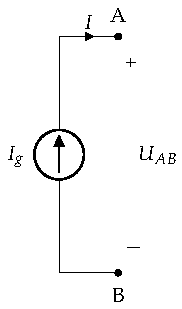
\includegraphics[height=3.5cm]{../figs/FuenteCorrienteIdeal.pdf}}\hfil
          \subfloat[Real]{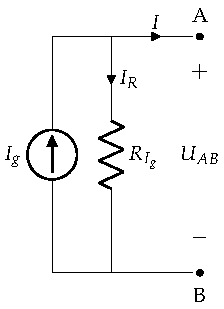
\includegraphics[height=3.5cm]{../figs/FuenteCorrienteRealDC.pdf}}
          \caption{Generador de corriente}
          \label{fig:fuentecorriente}
	\end{figure}
	
	\subsubsection{Dualidad de generadores}\label{sec.dualidad}
	
	Se dice que dos fuentes son equivalentes cuando suministran el
        \textbf{mismo valor de tensión y corriente} a un circuito
        externo, para cualquier circuito. Esta equivalencia solo puede
        darse entre \textbf{fuentes reales}.
	
	\begin{figure}[H]
          \centering \subfloat[Fuente real de
          tensión]{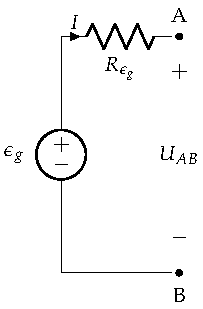
\includegraphics[height=4.9cm]{../figs/FuenteTensionRealDC.pdf}}\hfil
          \subfloat[Fuente real de
          corriente]{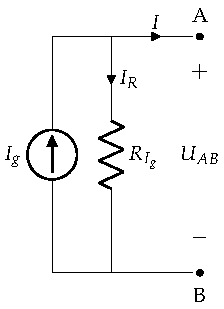
\includegraphics[height=4.9cm]{../figs/FuenteCorrienteRealDC.pdf}}
          \caption{Equivalencia de generadores}
          \label{fig:equivalencia_generadores}
	\end{figure}
	
	Considérense las fuentes de tensión y corriente, reales,
        mostradas en la Figura~\ref{fig:equivalencia_generadores} La
        salida de la fuente de tensión es:
	\begin{equation*}
          U_{AB} = \epsilon_g - R_{\epsilon_g} \cdot I
	\end{equation*}
	y la de la fuente de corriente:
	\begin{equation*}
          I = I_g - \frac{U_{AB}}{R_{I_g}} \rightarrow U_{AB} = R_{I_g} \cdot I_g - R_{I_g} \cdot I
	\end{equation*} 
	Por tanto, las fuentes son equivalentes cuando las ecuaciones
        coinciden para cualquier combinación de $(U_{AB}, I)$, es
        decir, si $R_g = R_{\epsilon_g} = R_{I_g}$:
	\begin{equation}\label{eq.equivalencia_fuentes}
          \boxed{\epsilon_g = R_{\epsilon_g} \cdot I_g \Leftrightarrow {I_g = \frac{\epsilon_g}{R_g}}}  
	\end{equation}
	
	\begin{remark}
          Nótese que el polo $+$ de la fuente de tensión queda en la
          misma posición que la flecha de la fuente de corriente
	\end{remark}
	
	\begin{example}\label{ex.1-2}
          \textbf{Convertir en fuente de intensidad o de tensión,
            según corresponda, las fuentes mostradas en la
            Figura~\ref{fig:ejemplo1-2}.}
          \begin{figure}[H]
            \centering
            \subfloat[]{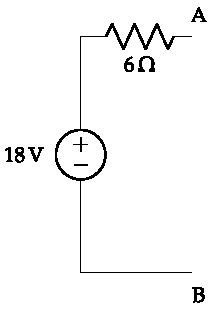
\includegraphics[height=3.5cm]{../figs/Conversion_Fuentes.pdf}}\hfil
            \subfloat[]{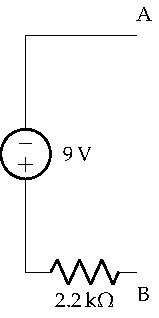
\includegraphics[height=3.5cm]{../figs/Conversion_Fuentes_2.pdf}}\hfil
            \subfloat[]{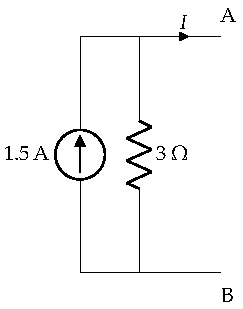
\includegraphics[height=3.5cm]{../figs/Conversion_Fuentes_3.pdf}}\hfil
            \subfloat[]{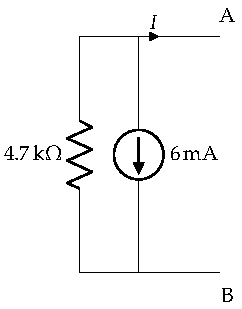
\includegraphics[height=3.5cm]{../figs/Conversion_Fuentes_4.pdf}}
            \caption{Ejemplo~\ref{ex.1-2}}
            \label{fig:ejemplo1-2}
          \end{figure}
	    
          \textbf{GENERADOR (a)}
	    
          Se puede transformar en un generador de corriente con una
          resistencia en paralelo de $6\Omega$, y de intensidad de la
          fuente $I_g=\frac{18}{6}=3$ A, con la punta de flecha hacia
          arriba.
	    
          \textbf{GENERADOR (b)}
	    
          Se puede transformar en un generador de corriente con una
          resistencia en paralelo de $2.2k\Omega$, y de intensidad de
          la fuente $I_g=\frac{9}{2.2\cdot10^3}=4.1$ mA, con la punta
          de flecha hacia abajo.
	    
          \textbf{GENERADOR (c)}
	    
          Se puede transformar en un generador de tensión con una
          resistencia en serie de $3\Omega$, y de fem de la fuente
          $\varepsilon_g=1.5\cdot 3=4.5$ V, con el polo $+$ arriba.
	    
          \textbf{GENERADOR (d)}
	    
          Se puede transformar en un generador de tensión con una
          resistencia en serie de $4.7k\Omega$, y de fem de la fuente
          $\varepsilon_g=6\cdot 10^{-3}\cdot 4.7\cdot 10^3=28.2$ V,
          con el polo $+$ abajo.
	\end{example}
        
        \subsubsection{Fuentes dominantes}
        \label{sec:dominancia}


        Por definición, una fuente de tensión ideal impone la tensión
        a su salida. Por tanto, todo aquello que esté conectado en
        paralelo con ella estará sometido a su tensión y, en
        consecuencia, el circuito equivalente estará compuesto
        únicamente por la fuente. En estas condiciones, se dice que
        una fuente de tensión es dominante sobre las ramas conectadas
        en paralelo (figura \ref{fig:fuente-tension-dominante}).

        De forma similar, una fuente de corriente impone la corriente
        que circula por su rama, por lo que los elementos conectados
        en serie pueden ser descartados para obtener un circuito
        equivalente. Por tanto, se dice que una fuente de corriente es
        dominante sobre los elementos conectados en serie (figura
        \ref{fig:fuente-corriente-dominante}).

        \begin{figure}
          \centering
          \subfloat[Fuente de
          tensión]{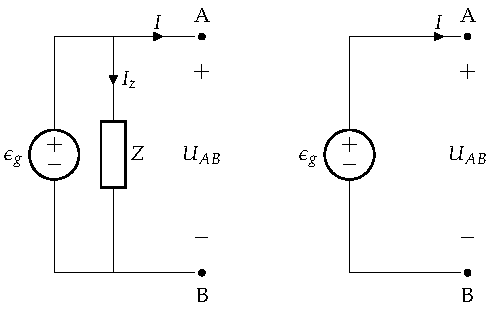
\includegraphics[height=4cm]{../figs/FuenteTensionDominante.pdf}\label{fig:fuente-tension-dominante}}\hfill
          \subfloat[Fuente de
          corriente]{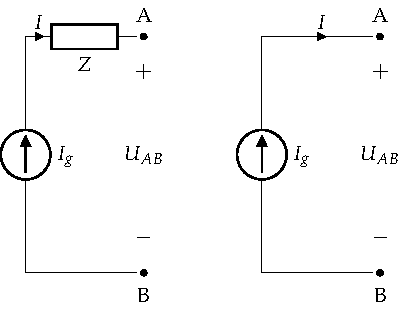
\includegraphics[height=4cm]{../figs/FuenteCorrienteDominante.pdf}\label{fig:fuente-corriente-dominante}}
          \caption{Generadores dominantes y sus circuitos
            equivalentes}
        \end{figure}

\subsubsection{Generadores dependientes o generadores controlados}
Pese a no ser estrictamente elementos activos, se comportan como
tales. Este tipo de generadores no tienen valores de $\epsilon$ o
$i_g$ fijos, sino que dependen de la tensión o corriente en otros
puntos de la red. Así, aparecen fundamentalmente cuatro tipos de
generadores dependientes, dependiendo de que cada generador suministre
una tensión o una corriente y según sea la variable de control una
tensión o una corriente. Estos generadores suelen representarse
mediante un rombo:
\begin{itemize}
\item \textbf{Generador de tensión controlado por tensión}
  (Figura~\ref{fig:tension-tension}): su tensión depende de la tensión
  entre otros puntos del circuito, siendo el parámetro $\alpha$
  adimensional [--]
\item \textbf{Generador de tensión controlado por corriente}
  (Figura~\ref{fig:tension-corriente}): su tensión depende de alguna
  corriente del circuito, teniendo el parámetro $\beta$ unidades de
  resistencia [$\Omega$]
\item \textbf{Generador de corriente controlado por tensión}
  (Figura~\ref{fig:corriente-tension}): su intensidad depende de la
  tensión entre dos puntos del circuito, teniendo el parámetro
  $\gamma$ unidades de conductancia [S]
\item \textbf{Generador de corriente controlado por corriente}
  (Figura~\ref{fig:corriente-corriente}): su intensidad es función de
  la corriente en otra parte del circuito, siendo el parámetro
  $\sigma$ adimensional [--]
\end{itemize}
\begin{figure}[H]
  \centering
  \subfloat[Tensión--Tensión]{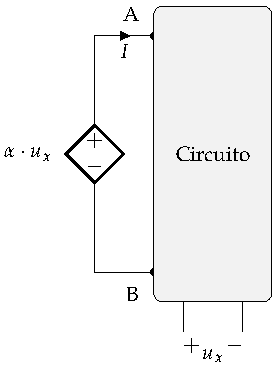
\includegraphics[height=4cm]{../figs/FuenteTensionDependienteTension.pdf}\label{fig:tension-tension}}\hfill
  \subfloat[Tensión--Corriente]{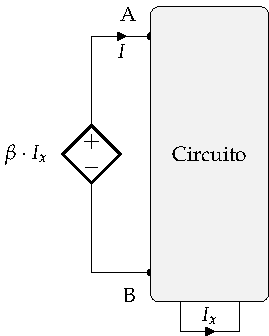
\includegraphics[height=4cm]{../figs/FuenteTensionDependienteCorriente.pdf}\label{fig:tension-corriente}}\hfill
  \subfloat[Corriente--Tensión]{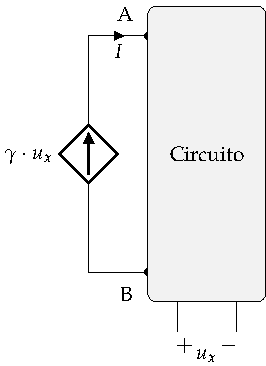
\includegraphics[height=4cm]{../figs/FuenteCorrienteDependienteTension.pdf}\label{fig:corriente-tension}}\hfill
  \subfloat[Corriente--Corriente]{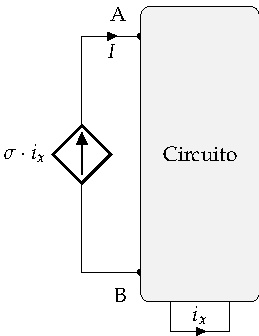
\includegraphics[height=4cm]{../figs/FuenteCorrienteDependienteCorriente.pdf}\label{fig:corriente-corriente}}
  \caption{Fuentes dependientes}
  \label{fig:fuentes_dependientes}
\end{figure}
	
	\begin{remark}
          Si en un circuito \textbf{solo} existen generadores
          dependientes, el circuito \textbf{no está excitado}.
	\end{remark}
	
	
	\subsubsection{Receptores}
	En este apartado se incluyen aquellos elementos activos que
        funcionan como receptores (absorben potencia del
        circuito). Estos elementos se caracterizan por su
        \textbf{fuerza contraelectromotriz} (f.c.e.m, E' o
        $\varepsilon'$), que es la energía por unidad de carga que
        transforman en otro tipo de energía que no sea calor. Al tener
        la misma naturaleza que la tensión eléctrica y la f.e.m.,
        también se mide en voltios [V]. Como en el caso de los
        generadores, se distingue entre receptor ideal y real
        (Figura~\ref{fig:receptores}):
	\begin{itemize}
        \item Un \textbf{receptor ideal} es aquel que \textbf{no tiene
            pérdidas}, de tal forma que la diferencia de potencial
          entre sus bornes toma siempre el mismo valor que su
          f.c.e.m. ($u_{AB}=\epsilon'$).
        \item Un \textbf{receptor real} es aquel que \textbf{tiene
            pérdidas}, caracterizadas mediante una resistencia
          interna, en \textbf{serie}, $R_{\epsilon'}$. Al circular una
          corriente por dicha resistencia, se consume en ella una
          potencia que no puede ser consumida por el receptor. Las
          pérdidas internas son la causa de que la diferencia de
          potencial entre sus bornes sea superior a la
          f.c.e.m. ($u_{AB}>\epsilon'$). Con esto, la potencia útil
          será $P_u=\epsilon'\cdot I$, la potencia disipada en la
          resistencia interna $P_p=R_{\epsilon'}\cdot I^2$ y la
          potencia absorbida $P_a=U_{AB}\cdot I$ y, dado que tiene que
          cumplirse el principio de conservación de la energía:
          \begin{equation}
            P_a=P_u+P_p\rightarrow \boxed{U_{AB}=\epsilon'+ R_{\epsilon'}\cdot I}\,
          \end{equation}
          \begin{figure}[H]
            \centering
            \subfloat[Ideal]{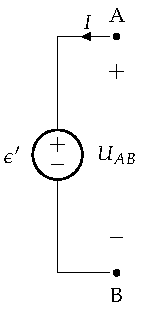
\includegraphics[height=3.5cm]{../figs/receptor_ideal.pdf}}\hfil
            \subfloat[Real]{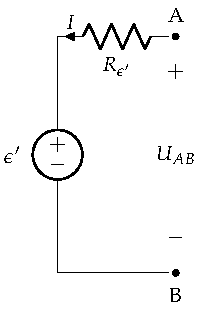
\includegraphics[height=3.5cm]{../figs/receptor_real.pdf}}
            \caption{Otros receptores}
            \label{fig:receptores}
          \end{figure}
	\end{itemize}
	

	\subsection{Eficiencia}
	Cualquier máquina, dispositivo, etc., tiene una
        \textbf{eficiencia}\footnote{No deben confundirse los términos
          de \textbf{eficiencia} y \textbf{rendimiento}. Mientras que
          eficiencia es la relación entre potencias, el rendimiento es
          la relación entre energías.} %(o eficiencia),
	que expresa el cociente entre la potencia de salida y la
        potencia de entrada. Puesto que todos los
        dispositivos/máquinas tienen pérdidas, se cumple
        \textbf{siempre} que el rendimiento es menor del 100\% (o 1,
        si se expresa en tanto por uno). En general, para la teoría de
        circuitos, interesa conocer el rendimiento de:
	\begin{itemize}
        \item Generadores:
          \begin{equation}
            \boxed{\eta_g (\%) = \frac{P_{u}}{P_{g}}\cdot 100}
          \end{equation}
        \item Receptores (fundamentalmente, motores):
          \begin{equation}
            \boxed{\eta_m (\%) = \frac{P_{u}}{P_{a}}\cdot 100}
          \end{equation}
	\end{itemize}
	
	\begin{example}\label{ex.motor-bt1}
          Un generador cuya \textit{fem} es de \qty{120}{\volt} y
          resistencia de \qty{0.2}{\ohm}, da una corriente de
          \qty{20}{\ampere} a un motor situado a \qty{300}{\meter} de
          distancia y de resistencia \qty{0.5}{\ohm}. La línea que los
          conecta es de cobre, de resistividad
          \qty{17.24}{\milli\ohm\milli\meter\squared\per\meter}. Sabiendo
          que el motor absorbe \qty{10.2}{\kWh} en \qty{5}{\hour}, se
          debe hallar: \vspace{3mm}

          \begin{enumerate}
          \item La fuerza contraelectromotriz (\textit{fcem}) del
            motor
          \item La sección de los conductores de la línea
          \item Los rendimientos de: motor, generador, línea y
            rendimiento total
          \item El balance general de potencias
          \end{enumerate}


          \hrulefill

          \vspace{5mm} \textbf{Solución}: \vspace{4mm}

          Empezamos dibujando el esquema del circuito y organizando
          los datos disponibles: \vspace{6mm}

          \begin{minipage}{0.68\linewidth}
            \begin{center}
              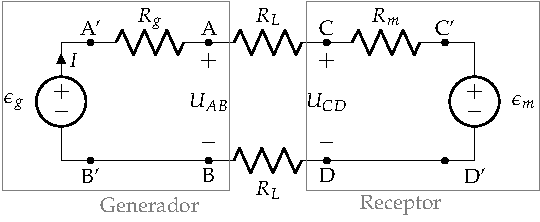
\includegraphics[scale=1]{../figs/circuito_lkv.pdf}
            \end{center}
          \end{minipage}
          \begin{minipage}{0.3\linewidth}
            \textbf{Datos}: \vspace{2mm}
  
            $\epsilon_g = \qty{120}{\volt}$\\
            $R_g = \qty{0.2}{\ohm}$\\
            $I = \qty{20}{\ampere}$\\
            $R_m = \qty{0.5}{\ohm}$\\
            $E_m = \qty{10.2}{\kWh}$ (en $\qty{5}{\hour}$)\\
            $l = \qty{300}{\meter}$\\
            $\rho =
            \qty{17.24}{\milli\ohm\milli\meter\squared\per\meter}$
          \end{minipage}

          \vspace{6mm}

          Donde la resistencia de la línea se divide en dos elementos,
          para distinguir entre el conductor de aporte y el de retorno
          de corriente.

          \vspace{6mm}

          \underline{Apartado 1}

          \vspace{4mm}

          Para calcular $\epsilon_m$, podemos formular el balance de
          tensiones (2LK) en la parte del motor:
          \[
            U_{CD} = \underbrace{I \cdot R_m}_{= 20 \cdot 0.5} +
            \epsilon_m
          \]

          Pero para despejar $\epsilon_m$ en la expresión anterior,
          necesitamos calcular $U_{CD}$.
          \begin{itemize}
          \item Opción 1: aplicar el balance de tensiones en la
            ``parte izquierda'' del circuito (a la izquierda de
            $U_{CD}$ en el diagrama).
    
            \underline{Problema}: no conocemos el valor de $R_L$ (y no
            podemos calcularlo usando la resistividad, porque
            desconocemos la sección de los conductores), luego no
            podemos calcular la caída de tensión en la línea.
    
          \item Opción 2: leyendo de nuevo la información que tenemos
            sobre el punto de operación del motor, vemos que es
            conocida la potencia absorbida por este.

    \[
      P_{CD} = \frac{10.2 \cdot 10^{3} \, \si{\Wh}}{\qty{5}{\hour}} =
      \qty{2040}{\watt}
    \]

    Luego:
    \[
      P_{CD} = U_{CD} \cdot I \quad \rightarrow \quad U_{CD} =
      \frac{2040}{20} = \qty{102}{\volt}
    \]

    Sustituyendo en la primera expresión:
    \[
      \epsilon_m = U_{CD} - 10 = \boxed{ \qty{92}{\volt} }
    \]

  \item Opción 3 (forma alternativa de llegar al resultado anterior):
    aplicar balance de potencias en el motor.
    \[
      P_{\textrm{útil}} = P_{\textrm{absorbida}} -
      P_{\textrm{pérdidas}} \quad \rightarrow \quad P_{\epsilon_m} =
      P_{CD} - \hspace{-3mm} \underbrace{P_{R_m}}_{\substack{= R_m
          \cdot I^2 \\[3pt] \text{(ley de Joule)}}}
    \]
    
    $P_{CD}$ se calcula de la forma descrita en la Opción 2, luego
    $P_{\epsilon_m}$ se obtiene como:
    \[
      P_{\epsilon_m} = 2040 - 0.5 \cdot 20^2 = \qty{1840}{\watt}
    \]

    Finalmente:
    \[
      P_{\epsilon_m} = \epsilon_m \cdot I \quad \rightarrow \quad
      \epsilon_m = \frac{1840}{20} = \boxed{ \qty{92}{\volt} }
    \]
  \end{itemize}

  \vspace{3mm}

  \underline{Apartado 2}

  \vspace{5mm}

  Para calcular la sección de la línea:
  \[
    R_L = \rho \cdot \frac{l}{S} = {17.24 \cdot
      10^{-3}}\si{\ohm\milli\meter\squared\per\meter} \cdot
    \frac{\qty{300}{\meter}}{S}
  \]
  (dado que ambos conductores, tanto el de aporte como el de retorno
  de corriente, tienen una $l=\qty{300}{\meter}$ cada uno)

  \vspace{3mm} Luego debemos calcular el valor de $R_L$ para poder
  despejar $S$.
  \begin{itemize}
  \item Opción 1: aplicar el balance de tensiones en todo el circuito
    (2LK). Comenzando en el punto $A$, y retornando al mismo punto:
    
    \[
      R_L \cdot I + U_{CD} + R_L \cdot I - \epsilon_g + R_g \cdot I =
      0
    \]
    Despejando $R_L$:
    \[
      2 R_L \cdot I = \underbrace{\epsilon_g}_{=\qty{120}{\volt}} -
      \underbrace{R_g \cdot I}_{=0.2 \cdot 20} -
      \underbrace{U_{CD}}_{=\qty{102}{\volt}} \quad \rightarrow \quad
      \boxed{ R_L = {\frac{7}{20}}\si{\ohm} }
    \]

  \item Opción 2: aplicar balance de potencias en la línea.

    \vspace{2mm}
    \begin{minipage}{0.4\linewidth}
      \begin{center}
        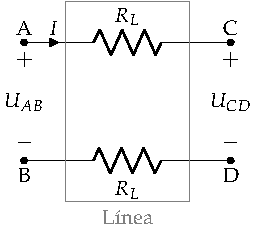
\includegraphics[scale=1]{../figs/linea_lkv.pdf}
      \end{center}
    \end{minipage}
    \begin{minipage}{0.6\linewidth}
      \begin{align*}
        P_{\textrm{entrada}} &= P_{\textrm{pérdidas línea}} + P_{\textrm{salida}}\\[10pt]
        U_{AB} \cdot I &= 2 \cdot R_L \cdot I^2 + U_{CD} \cdot I\\[10pt] 
        R_L &= \frac{U_{AB}-U_{CD}}{2 \cdot I} \underarrow[=][\uparrow]{\small 2LK para \ensuremath{U_{AB}} } \frac{\epsilon_g - I\cdot R_g - 102}{2 \cdot 20} = \Aboxed{ {\frac{7}{20}}\si{\ohm} }
        % Flecha, sacada de aquí:
        % https://tex.stackexchange.com/questions/8720/overbrace-underbrace-but-with-an-arrow-instead
        % Sin "\ensuremath" da error al meter un símbolo matemático
      \end{align*}
    \end{minipage}
  \end{itemize}

  Una vez conocemos el valor de $R_L$, despejamos $S$ en la primera
  expresión:

\[
  S = \rho \cdot \frac{l}{R_L} = \boxed{
    \qty{14.78}{\milli\meter\squared} }
\]

Dado que este valor no corresponde a una sección normalizada de cable,
en la práctica este circuito contendría un cable de sección
normalizada inmediatamente superior a este valor, es decir, de
$S = \qty{16}{\milli\meter\squared}$.

\vspace{6mm}

\underline{Apartado 3}

\vspace{5mm}

Los rendimientos pedidos se calculan de la siguiente forma:
\begin{align*}
  \eta_m &= \frac{P_{\textrm{útil}}}{P_{\textrm{absorbida}}} = \frac{\epsilon_m \cdot \bcancel{I}}{U_{CD} \cdot \bcancel{I}} = \frac{\qty{92}{\volt}}{\qty{102}{\volt}}  = \boxed{0.902}\\[10pt]
  \eta_g &= \frac{P_{\textrm{entregada}}}{P_{\textrm{producida}}} = \frac{U_{AB}}{\epsilon_g} = \frac{\qty{116}{\volt}}{\qty{120}{\volt}} = \boxed{0.967}\\[10pt]
  \eta_{\textrm{línea}} &= \frac{P_{\textrm{salida}}}{P_{\textrm{entrada}}} = \frac{U_{CD}}{U_{AB}} = \frac{\qty{102}{\volt}}{\qty{116}{\volt}} = \boxed{0.879}\\[10pt]
  \eta_{\textrm{total}} &= \frac{P_{\textrm{útil}}}{P_{\textrm{producida}}} = \frac{\epsilon_m}{\epsilon_g} = \frac{\qty{92}{\volt}}{\qty{120}{\volt}} = \eta_g \cdot \eta_{\textrm{línea}} \cdot \eta_m = \boxed{0.767}
\end{align*}

\vspace{2mm}

\underline{Apartado 4}

\vspace{5mm}

El balance de potencias del circuito es:

\[
  P_{g} = P_{\textrm{línea}} + P_{m}
\]

Donde:

\vspace{-3mm}
\begin{align*}
  & P_{g} = P_{\textrm{útil}, \, g} + P_{\textrm{pérdidas}, \, g} & \rightarrow \qquad & \epsilon_g \cdot I = U_{AB} \cdot I + R_g \cdot I^2 \\[10pt]
  & P_{\textrm{línea}} = P_{\textrm{útil, línea}} + P_{\textrm{pérdidas, línea}} \hspace{-20mm} & \rightarrow \qquad & U_{AB} \cdot I = U_{CD} \cdot I + 2 R_L \cdot I^2\\[10pt]
  & P_{m} = P_{\textrm{útil}, \, m} + P_{\textrm{pérdidas}, \, m} & \rightarrow \qquad & U_{CD} \cdot I = \epsilon_m \cdot I + R_m \cdot I^2 
\end{align*}
	    
\end{example}



\begin{example}\label{ex.motor2-bt1}

  Un generador de corriente continua alimenta dos cargas. La primera
  de estas cargas está situada a \qty{2100}{\meter} del generador,
  tiene una resistencia de \qty{215}{\ohm} y rendimiento unidad. La
  segunda carga está situada \qty{270}{\meter} después de la primera,
  tiene una potencia de \qty{4662}{\watt}, un rendimiento del 75\% y
  una tensión aplicada de \qty{420}{\volt}.  La línea es de cobre, de
  \qty{6}{\milli\meter\squared} de sección y con una resistividad de
  \qty{17.24}{\milli\ohm\milli\meter\squared\per\meter}.
    
  \vspace{2mm}
    
  Con esta información, se debe calcular:
    
  \begin{enumerate}
  \item La tensión en bornes del generador
  \item La corriente entregada por el generador
  \item El rendimiento de la instalación
  \end{enumerate}
    
  \hrulefill

  \vspace{5mm} \textbf{Solución}: \vspace{4mm}

  Empezamos dibujando el esquema del circuito y organizando los datos
  disponibles: \vspace{6mm}
    
    \begin{minipage}{0.725\linewidth}
      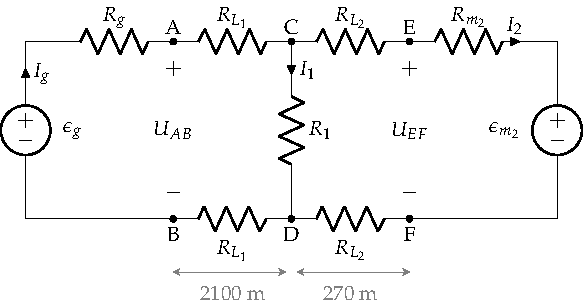
\includegraphics[scale=1]{../figs/circuito_ejercicio2_BT1.pdf}
    \end{minipage}
    \begin{minipage}{0.275\linewidth}
    
      \vspace{-5mm} \textbf{Datos}:
      
      \vspace{2mm}
    
      $l_1 = \qty{2100}{\meter}$\\
      $R_1 = \qty{215}{\ohm}$\\
      $\eta_1 = 100\%$\\
      $l_2 = \qty{270}{\meter}$\\
      $P_2 = \qty{4662}{\watt}$\\
      $\eta_2 = 75\%$\\
      $U_{EF} = \qty{420}{\volt}$\\
      $\rho_L = \qty{17.24}{\milli\ohm\milli\meter\squared\per\meter}$\\
      $S_L = \qty{6}{\milli\meter\squared}$
    \end{minipage}
    
    \vspace{6mm}
    
    Unos apuntes sobre la información de que disponemos:
    \begin{itemize}
    \item Dado que la primera de las cargas tiene rendimiento unidad,
      toda la potencia que recibe es potencia útil. Al tener esta
      carga una resistencia, para que pueda tener un rendimiento del
      100\%, esta carga es necesariamente una \underline{resistencia
        pura}. Aunque típicamente usamos las resistencias para modelar
      pérdidas de energía por efecto Joule, en este caso la usamos
      para modelar calor como trabajo útil: esta carga podría
      representar, por ejemplo, un calefactor, cuya función es
      producir calor.
    \item Dado que la segunda carga tiene un rendimiento menor que la
      unidad, sabemos que no es un motor ideal, por lo que debemos
      incluir su resistencia interna, $R_{m_2}$.
    \item La potencia de la segunda carga, $P_2 = \qty{4662}{\watt}$,
      es su potencia útil.
    \item Dado que la tensión aplicada en la segunda carga es de
      \qty{420}{\volt}, esto implica que $U_{EF} = \qty{420}{\volt}$.
    \item Dado que hay dos nudos en el circuito (C y D), no hay una
      única corriente, sino tres distintas ($I_g, \, I_1, \, I_2$).
    \item En cuanto al generador: no tenemos información suficiente
      para saber si se trata de un generador ideal o real. Es
      recomendable asumir incialmente que es real, y si al resolver el
      problema llegamos a la conclusión de que $R_g=\qty{0}{\ohm}$,
      entonces se tratará de un generador ideal.
    \end{itemize}
    
    
    \vspace{3mm}
    
    \underline{Apartado 1}
    
    \vspace{4mm}
    
    Debemos calcular la tensión en bornes del generador, es decir, la
    tensión a la salida del mismo, $U_{AB}$.
    
    Podemos hacerlo aplicando 2LK, una vez conozcamos $U_{AC}$ y
    $U_{CD}$ (dado que $U_{AC} = U_{DB}$). Para obtener estos valores:
    \begin{itemize}
    \item Para calcular $U_{CD}$ es necesario conocer el valor de
      $R_{L_2}$ e $I_2$:
    
      Tenemos información sobre la carga 2: dado que conocemos su
      potencia útil y rendimiento, podemos calcular su potencia
      absorbida. Con la potencia absorbida, y usando la tensión a la
      entrada del motor, podemos calcular la corriente absorbida por
      este:
        
        \[
          \eta_m = \frac{P_{\textrm{útil}}}{P_{\textrm{absorbida}}} =
          \frac{\qty{4662}{\watt}}{U_{EF} \cdot I_2} =
          \frac{4662}{420\cdot I_2} = 0.75 \quad \rightarrow \quad I_2
          = \qty{14.8}{\ampere}
        \]
    
        Una vez calculemos el valor de $R_{L_2}$, y conociendo ya la
        corriente $I_2$ que circula por ellas, podemos calcular la
        caída de tensión en la línea 2, y finalmente obtener $U_{CD}$:
    
        \[
          R_{L_2} = \rho \cdot \frac{l}{S} = {17.24 \cdot 10^{-3}}
          \cdot \frac{270}{6} = \qty{0.78}{\ohm}
        \]
        
        \vspace{-10mm}
        \[
          U_{CD} \overarrow[=][\downarrow]{\small 2LK} U_{CE} + U_{EF}
          + U_{FD} = R_{L_2}\cdot I_2 + 420 + R_{L_2}\cdot I_2 =
          \qty{443.09}{\volt}
          % Flecha, sacada de aquí:
          % https://tex.stackexchange.com/questions/8720/overbrace-underbrace-but-with-an-arrow-instead
        \]
    
      \item Para calcular $U_{AC}$ necesitamos conocer tanto $R_{L_1}$
        como $I_g$:
    
        \vspace{-7mm}
        \[
          I_1 = \frac{U_{CD}}{R_1} = \frac{443.09}{215} =
          \qty{2.06}{\ampere} \;\; \text{\small (ley de Ohm)} \quad
          \rightarrow \quad I_g \overarrow[=][\downarrow]{\small 1LK}
          I_1 + I_2 = 2.06 + 14.8 = \qty{16.86}{\ampere}
        \]
        \[
          R_{L_1} = \rho \cdot \frac{l}{S} = {17.24 \cdot 10^{-3}}
          \cdot \frac{2100}{6} = \qty{6.03}{\ohm}
        \]
    
        \vspace{-9mm}
        \[
          U_{AB} \overarrow[=][\downarrow]{\small 2LK} U_{AC} + U_{CD}
          + U_{BD} = R_{L_1}\cdot I_g + 443.09 + R_{L_1}\cdot I_g =
          \boxed{ \qty{646.42}{\volt} }
          % Flecha, sacada de aquí:
          % https://tex.stackexchange.com/questions/8720/overbrace-underbrace-but-with-an-arrow-instead
        \]
        
      \end{itemize}
    
    
      \vspace{2mm}
    
      \underline{Apartado 2}
    
      \vspace{4mm}
    
      $I_g$ ya ha sido calculada en el apartado anterior, aplicando
      1LK:
    
    \[
      I_g = I_1 + I_2 = 2.06 + 14.8 = \boxed{ \qty{16.86}{\ampere} }
    \]
    
    \vspace{2mm}
    
    \underline{Apartado 3}
    
    \vspace{-3mm}
    
    \[
      \eta_{\textrm{total}} =
      \frac{P_{\textrm{útil}}}{P_{\textrm{producida}}} =
      \frac{R_1\cdot I_1^2 + \epsilon_{m_2} \cdot I_2}{U_{AB} \cdot
        I_g} = \frac{215 \cdot 2.06^2 + \overbrace{\eta_2 \cdot
          U_{EF}}^{=0.75\cdot 420} \cdot 14.8}{646.42 \cdot 16.86} =
      \boxed{51.15\%}
    \]
    
    Nota: este rendimiento asume que el generador es ideal, dado que
    no conocemos su resistencia interna, y por lo tanto no podemos
    calcular sus pérdidas por efecto Joule.

    \vspace{2mm} Aunque el ejercicio ya está resuelto, vamos a
    calcular el rendimiento de cada elemento para entender mejor dónde
    ocurren las pérdidas en el circuito:

    \vspace{-3mm}
    \begin{align*}
      \eta_{L_1} &= \frac{P_{\textrm{salida}}}{P_{\textrm{entrada}}} = \frac{U_{CD}\cdot \bcancel{I_g}}{U_{AB} \cdot \bcancel{I_g}} = \frac{443.09}{646.42} = 68.55\%\\[10pt]
      \eta_{R_1} &= 100\% \;\; \text{(dado en el enunciado)}\\[10pt]
      \eta_{L_2} &= \frac{P_{\textrm{salida}}}{P_{\textrm{entrada}}} = \frac{U_{EF}}{U_{CD}} = \frac{420}{443.09} = 94.79\%\\[10pt]
      \eta_{m_2} &= 75\% \;\; \text{(dado en el enunciado)}  
    \end{align*}
    
    Vemos que la línea 1 tiene unas pérdidas enormes, debidas a su
    gran longitud. Las pérdidas podrían reducirse eligiendo un
    conductor con una sección mayor, que haría disminuir la
    resistencia de la línea.

  \end{example}


	
  \section{Asociación de elementos}
	
  Los diferentes elementos (tanto los activos como los pasivos) se
  pueden asociar de diferentes formas según la conexión que se haga
  entre ellos.
	
	\subsection{Conexión en serie}
	Se dice que dos o más elementos están acoplados en
        \textbf{serie} cuando el final del primero se conecta al
        principio del segundo, el final del segundo al principio del
        tercero, y así sucesivamente. Es decir, varios elementos están
        conectados en serie cuando por ellos circula la \textbf{misma
          corriente}.
	
	\subsubsection{Resistencias}
	Siguiendo el circuito de la Figura~\ref{fig:serie}, se cumple
        que:
        \begin{align*}
          u_1(t) &= R_1 \cdot i(t)\\
          u_2(t) &= R_2 \cdot i(t)\\
          u_3(t) &= R_3 \cdot i(t)
        \end{align*}
        \begin{figure}[H]
          \centering
          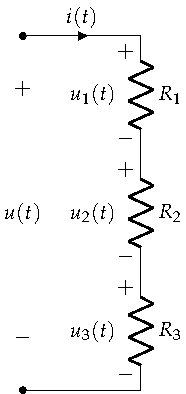
\includegraphics[width=0.2\linewidth]{../figs/AsociacionSerie.pdf}
          \caption{Conexión de resistencias en serie}
          \label{fig:serie}
        \end{figure}
        Al aplicar la 2LK, se obtiene que:
        \begin{equation*}
          u(t) = u_1(t) + u_2(t) + u_3(t)
        \end{equation*}
        y sacando $i(t)$ como factor común, queda:
        \begin{equation*}
          u(t) = i(t) \cdot (R_1 + R_2 + R_3)
        \end{equation*}
        Por tanto, se puede definir la resistencia equivalente
        $R_{eq}$ de la conexión en serie como:
        \begin{equation}
          \boxed{R_{eq} = \sum_{i = 1}^n R_i}
        \end{equation}
        de modo que:
        \begin{equation*}
          u(t) = R_{eq} \cdot i(t)
        \end{equation*}
		
        Además, de las ecuaciones anteriores se tiene:
        \begin{align*}
          i(t) = \dfrac{u(t)}{R_1 + R_2 + R_3}
        \end{align*}
        pudiendo calcular la tensión de cualquiera de las resistencias
        como:
        \begin{equation*}
          u_i(t) = R_i \cdot i(t)
        \end{equation*}
        Por tanto, la tensión parcial $u_i(t)$ se puede expresar en
        función de la tensión total $u(t)$ como:
        \begin{equation*}
          u_i(t) = u(t) \cdot \frac{R_i}{R_1 + R_2 + R_3}
        \end{equation*}
        conocido como \textbf{divisor de tensión}. En general, para un
        circuito en serie:
        \begin{equation}
          \boxed{u_i(t) = u(t) \cdot \frac{R_i}{R_{eq}}}
        \end{equation}
        \subsubsection{Bobinas}
        Siguiendo el circuito de la Figura~\ref{fig:bobinas-serie}, se
        cumple que:
        \begin{align*}
          u_1(t) &= L_1 \cdot \dfrac{di(t)}{dt}\\
          u_2(t) &= L_2 \cdot \dfrac{di(t)}{dt}\\
          u_3(t) &= L_3 \cdot \dfrac{di(t)}{dt}\\
        \end{align*}
        \begin{figure}[H]
          \centering
          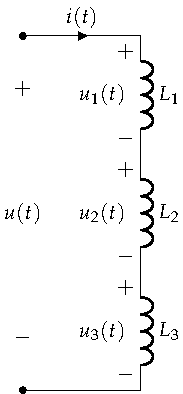
\includegraphics[width=0.2\linewidth]{../figs/BobinasSerie.pdf}
          \caption{Conexión de bobinas en serie}
          \label{fig:bobinas-serie}
        \end{figure}
        De manera análoga a las resistencias, al aplicar la 2LK se
        obtiene que:
        \begin{equation*}
          u(t) = u_1(t) + u_2(t) + u_3(t)
        \end{equation*}
        y sacando $\frac{di(t)}{dt}$ como factor común, queda:
        \begin{equation*}
          u(t) = \dfrac{di(t)}{dt} \cdot (L_1 + L_2 + L_3)
        \end{equation*}
        por lo que se puede definir la inductancia equivalente
        $L_{eq}$ de la conexión en serie como:
        \begin{equation}
          \boxed{L_{eq} = \sum_{i = 1}^n L_i}
        \end{equation}
        de modo que:
        \begin{equation*}
          u(t) = L_{eq} \cdot \dfrac{di(t)}{dt}
        \end{equation*}
        \subsubsection{Condensadores}
        Con el circuito de la Figura~\ref{fig:condensadores-serie}, se
        cumple que:
        \begin{align*}
          i(t) &= C_1 \cdot \frac{du_1(t)}{dt}\\
          i(t) &= C_2 \cdot \frac{du_2(t)}{dt}\\
          i(t) &= C_3 \cdot \frac{du_3(t)}{dt}\\
        \end{align*}
        \begin{figure}[H]
          \centering
          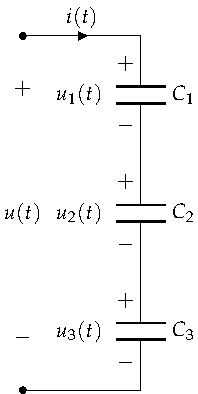
\includegraphics[width=0.2\linewidth]{../figs/CondensadoresSerie.pdf}
          \caption{Conexión de condensadores en serie}
          \label{fig:condensadores-serie}
        \end{figure}
        Al aplicar la 2LK se obtiene que:
        \begin{equation*}
          u(t) = u_1(t) + u_2(t) + u_3(t)
        \end{equation*}
        Suponiendo que la carga sea nula en el instante inicial (para
        que las constantes de integración sean nulas) y sacando factor
        común $\int i(t)\,dt$, se tiene:
        \begin{equation*}
          u(t)=\left(\dfrac{1}{C_1}+\dfrac{1}{C_2}+\dfrac{1}{C_3} \right)\cdot \int i(t) dt
        \end{equation*}
        por lo que se puede definir la capacidad equivalente $C_{eq}$
        de la conexión en serie como:
        \begin{equation}
          \boxed{\dfrac{1}{C_{eq}} = \sum_{i = 1}^n \dfrac{1}{C_i}}
        \end{equation}
        de modo que:
        \begin{equation*}
          i(t) = C_{eq} \cdot \frac{du(t)}{dt}
        \end{equation*}
		
        \subsubsection{Fuentes de tensión}
		
        Pueden conectarse en serie sin que exista \textbf{ninguna
          restricción}, independientemente de que se considere su
        modelo ideal o real. Su f.e.m. equivalente será la suma de
        cada una de las f.e.m.s. (por la 2LK) y, la resistencia
        equivalente, la suma de las resistencias internas de cada
        generador (en caso de considerar el modelo real).
		
        \subsubsection{Fuentes de corriente}
		
        Hay que hacer diferencia entre si se considera el modelo ideal
        o el real:
        \begin{itemize}
        \item \textbf{Ideal.} Las fuentes de corriente ideales pueden
          conectarse en serie si, y sólo si, todas las fuentes
          suministran \textbf{igual intensidad y en el mismo sentido}
          (por la 1LK).
        \item \textbf{Real.} No existe ninguna restricción, llegando
          al generador equivalente mediante trasformación de fuentes
          (ver Sección~\ref{sec.dualidad}).
        \end{itemize}
	
	\subsection{Conexión en paralelo}
	Se dice que dos o más elementos están acoplados en
        \textbf{paralelo} cuando todos los principios están conectados
        a un mismo punto, y todos los finales lo están en otro. Es
        decir, varios elementos están conectados en paralelo cuando
        todos ellos se encuentran sometidos a la \textbf{misma
          diferencia de potencial}.
	
        \subsubsection{Resistencias}
			
        Con el circuito de la Figura~\ref{fig:resistencias-paralelo},
        se cumple que:
        \begin{align*}
          i_1(t) &= \dfrac{u(t)}{R_1}\\
          i_2(t) &= \dfrac{u(t)}{R_2}\\
          i_3(t) &= \dfrac{u(t)}{R_3}\\
        \end{align*}
        \begin{figure}[H]
          \centering
          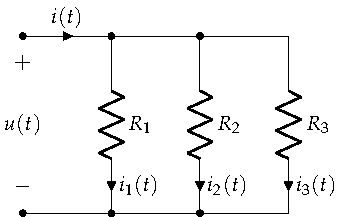
\includegraphics[width=0.35\linewidth]{../figs/AsociacionParalelo.pdf}
          \caption{Conexión de resistencias en paralelo}
          \label{fig:resistencias-paralelo}
        \end{figure}
        Al aplicar la 1LK, se obtiene que:
        \begin{equation*}
          i(t) = i_1(t) + i_2(t) + i_3(t)
        \end{equation*}
        y sacando $u(t)$ como factor común, queda:
        \begin{equation*}
          i(t) = u(t) \cdot \left(\frac{1}{R_1} + \frac{1}{R_2} + \frac{1}{R_3}\right)
        \end{equation*}
        Por tanto, se puede definir la resistencia equivalente
        $R_{eq}$ de la conexión en paralelo como:
        \begin{equation}
          \boxed{\dfrac{1}{R_{eq}} = \sum_{i = 1}^n \dfrac{1}{R_i}}
        \end{equation}
        de modo que:
        \begin{equation*}
          u(t) = R_{eq} \cdot i(t)
        \end{equation*}
		
		\begin{remark}
                  En el caso concreto de \textbf{dos resistencias} en
                  paralelo, la expresión sería:
                  \begin{equation*}
                    R_{eq}=\dfrac{1}{\frac{1}{R_1}+\frac{1}{R_2}}=\dfrac{1}{\frac{R_2+R_1}{R_1\cdot R_2}}=\dfrac{R_1\cdot R_2}{R_1+R_2}
                  \end{equation*}
		\end{remark}
		
		Se define la \textbf{conductancia} $G$ [S] como la
                inversa de la resistencia. Así, en lugar de:
		\begin{equation*}
                  \dfrac{1}{R_{eq}} = \sum_{i = 1}^n \dfrac{1}{R_i}
		\end{equation*}
		\begin{equation*}
                  u(t) = R_{eq} \cdot i(t)
		\end{equation*}
		se puede escribir:
		\begin{equation}
                  \boxed{G_{eq} = \sum_{i = 1}^n G_i}
		\end{equation}
		\begin{equation*}
                  i(t) = G_{eq} \cdot u(t)
		\end{equation*}
		
		Además, de las ecuaciones anteriores (usando la
                conductancia) se tiene:
		\begin{align*}
                  u(t) = \dfrac{i(t)}{G_1 + G_2 + G_3}
		\end{align*}
		pudiendo calcular la corriente de cualquiera de las
                resistencias como:
		\begin{equation*}
                  i_i(t) = G_i \cdot u(t)
		\end{equation*}
		Por tanto, la corriente parcial $i_i(t)$ se puede
                expresar en función de la corriente total $i(t)$ como:
		\begin{equation*}
                  i_i(t) = i(t) \cdot \dfrac{G_i}{G_1 + G_2 + G_3}
		\end{equation*}
		conocido como \textbf{divisor de corriente}. En
                general, para un circuito en paralelo:
		\begin{equation}
                  \boxed{i_i(t) = i(t) \cdot \frac{G_i}{G_{eq}}}
		\end{equation}
		
		\subsubsection{Bobinas}
		
		Considerando el circuito de la
                Figura~\ref{fig:bobinas-paralelo}, se cumple que:
		\begin{align*}
                  u(t) &= L_1 \cdot \frac{di_1(t)}{dt}\\
                  u(t) &= L_2 \cdot \frac{di_2(t)}{dt}\\
                  u(t) &= L_3 \cdot \frac{di_3(t)}{dt}\\
		\end{align*}
		\begin{figure}[H]
                  \centering
                  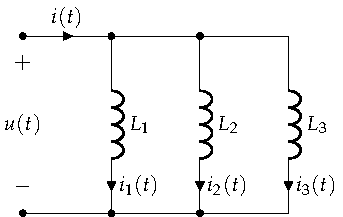
\includegraphics[width=0.35\linewidth]{../figs/BobinasParalelo.pdf}
                  \caption{Conexión de bobinas en paralelo}
                  \label{fig:bobinas-paralelo}
		\end{figure}
		Al aplicar la 1LK, se obtiene que:
		\begin{equation*}
                  i(t) = i_1(t) + i_2(t) + i_3(t)
		\end{equation*}
		y, suponiendo que la carga sea nula en el instante
                inicial (para que las constantes de integración sean
                nulas) y sacando factor común $\int u(t)\,dt$, se
                tiene:
		\begin{equation*}
                  i(t)=\left(\dfrac{1}{L_1}+\dfrac{1}{L_2}+\dfrac{1}{L_3} \right)\cdot \int u(t) dt
		\end{equation*}
		Por tanto, se puede definir la inductancia equivalente
                $L_{eq}$ de la conexión en paralelo como:
		\begin{equation}
                  \boxed{\dfrac{1}{L_{eq}} = \sum_{i = 1}^n \dfrac{1}{L_i}}
		\end{equation}
		de manera que:
		\begin{equation*}
                  u(t) = L_{eq} \cdot \dfrac{di(t)}{dt}
		\end{equation*}
		\subsubsection{Condensadores}
		Con el circuito de la
                Figura~\ref{fig:condensadores-paralelo}, se cumple
                que:
		\begin{align*}
                  i_1(t) &= C_1 \cdot \frac{du(t)}{dt}\\
                  i_2(t) &= C_2 \cdot \frac{du(t)}{dt}\\
                  i_3(t) &= C_3 \cdot \frac{du(t)}{dt}\\
		\end{align*}
		\begin{figure}[H]
                  \centering
                  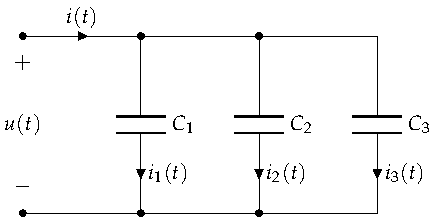
\includegraphics[width=0.4\linewidth]{../figs/CondensadoresParalelo.pdf}
                  \caption{Conexión de condensadores en paralelo}
                  \label{fig:condensadores-paralelo}
		\end{figure}
		Al aplicar la 1LK se obtiene que:
		\begin{equation*}
                  i(t) = i_1(t) + i_2(t) + i_3(t)
		\end{equation*}
		por lo que, sacando factor común $\frac{du(t)}{dt}$,
                se tiene:
		\begin{equation*}
                  i(t)=C_1\cdot \dfrac{du(t)}{dt}+ C_2\cdot \dfrac{du(t)}{dt}+ C_3\cdot \dfrac{du(t)}{dt}=(C_1+C_2+C_3)\cdot\dfrac{du(t)}{dt}
		\end{equation*}
		por lo que se puede definir la capacidad equivalente
                $C_{eq}$ de la conexión en paralelo como:
		\begin{equation}
                  \boxed{C_{eq} = \sum_{i = 1}^n C_i}
		\end{equation}
		de modo que:
		\begin{equation*}
                  i(t) = C_{eq} \cdot \frac{du(t)}{dt}
		\end{equation*}
		
		\subsubsection{Fuentes de tensión}
		
		Hay que hacer diferencia entre si se considera el
                modelo ideal o el real:
		\begin{itemize}
                \item \textbf{Ideal.} Las fuentes de tensión ideales
                  pueden conectarse en paralelo si, y sólo si, todas
                  las fuentes tienen \textbf{igual f.e.m. y ésta actúa
                    en el mismo sentido}.
                \item \textbf{Real.} No existe \textbf{ninguna
                    restricción}, llegando al generador equivalente
                  mediante trasformación de fuentes (ver
                  Sección~\ref{sec.dualidad}).
		\end{itemize}
		
		\subsubsection{Fuentes de corriente}
		
		Pueden conectarse en paralelo sin que exista ninguna
                restricción, independientemente de que se considere su
                modelo ideal o real. Su intensidad equivalente será la
                suma de cada una de las intensidades, y la resistencia
                equivalente se calculará a partir del paralelo entre
                varias resistencias (en caso de considerar el modelo
                real).
	
	
	\begin{example}\label{ex.serie-paralelo}
          \textbf{Calcular la corriente que pasa por la fuente de
            tensión de la Figura \ref{fig:ejercicio1_tema1}.}
          \begin{figure}[H]
            \centering 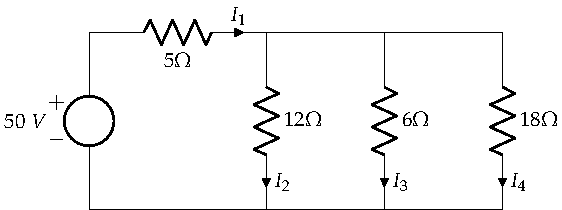
\includegraphics{../figs/ej1_BT1.pdf}
            \caption{Ejemplo~\ref{ex.serie-paralelo}}
            \label{fig:ejercicio1_tema1}
          \end{figure}
		
          Se pide calcular la corriente $I_1$. Se empiezan asociando
          las tres resistencias en paralelo de 12, 6 y 18~$\Omega$:
          \begin{equation*}
            R_{eq,||}=\dfrac{1}{\frac{1}{R_{12}}+\frac{1}{R_{6}}+\frac{1}{R_{18}}}=\dfrac{1}{\frac{1}{12}+\frac{1}{6}+\frac{1}{18}}=3.273\,\Omega
          \end{equation*}
          La resistencia equivalente total:
          \begin{equation*}
            R_{eq}=R_5+R_{eq,||}=5+3.273=8.273\,\Omega
          \end{equation*}
          Por la ley de Ohm:
          \begin{equation*}
            I_1=\dfrac{U}{R_{eq}}=\dfrac{50}{8.273}={6.04\,\text{A}}
          \end{equation*}
	\end{example}
	
	
	
	\subsection{Conexión estrella-triángulo}
	Estas dos configuraciones tienen una importancia fundamental
        en la teoría de circuitos, ya que son las dos posibilidades de
        conexión de cargas trifásicas. En la
        Figura~\ref{fig:estrella-triangulo} se muestran estas redes
        pasivas, cuyos terminales de acceso exterior se han denominado
        $A$, $B$ y $C$ y que tienen la misma situación
        ``topográfica''. La conexión triángulo está formada por tres
        resistencias $R_{ab}$, $R_{bc}$ y $R_{ca}$, que unen los
        diversos nudos, dando la apariencia geométrica de un
        triángulo. Por su parte, la conexión estrella representa tres
        resistencias $R_a$, $R_b$ y $R_c$, que parten de los tres
        nudos de acceso externo $A$, $B$ y $C$, y que se unen en un
        punto común $N$.
	\begin{figure}[H]
          \centering \subfloat[Conexión
          triángulo]{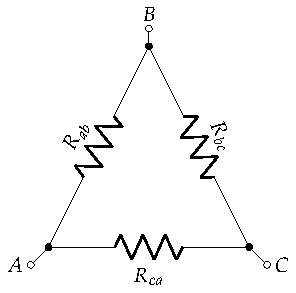
\includegraphics[width=0.3\linewidth]{../figs/Conexion_Triangulo.pdf}}\hfil
          \subfloat[Conexión
          estrella]{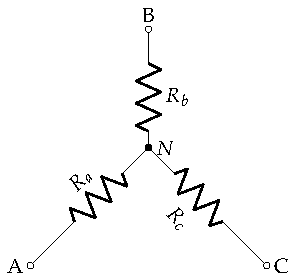
\includegraphics[width=0.3\linewidth]{../figs/Conexion_Estrella.pdf}}
          \caption{Conexión en estrella y en triángulo}
          \label{fig:estrella-triangulo}
	\end{figure}
	
	Lo interesante es buscar las leyes de transformación de una
        red a la otra, de tal modo que ambos circuitos sean
        equivalentes desde el punto de vista externo (es decir, desde
        los nudos $A$, $B$ y $C$). Está claro que, si las dos redes
        son equivalentes, deberán consumir las mismas corrientes
        cuando se aplican las mismas tensiones externas, lo que
        equivale a decir que las resistencias que se observan entre
        los diferentes terminales $A-B$, $B-C$ y $C-A$ deben ser
        idénticas para ambos montajes y, por consiguiente, se deben
        satisfacer las igualdades mostradas en la
        Tabla~\ref{tab.igualdades_estrellatriangulo}.
	\begin{table}[H]
          \centering
          \begin{tabular}{c|c|c} \textbf{Resistencia} &
            \textbf{Estrella} & \textbf{Triángulo}\\\hline
                                                      &&        \\[-0.75em]
            $R_{AB}$ & $R_a+R_b$ & $\dfrac{R_{ab} \cdot (R_{bc} + R_{ca})}{R_{ab} + R_{bc} + R_{ca}}$\\
                                                      &&         \\[-0.75em]
            $R_{AB}$ & $R_b+R_c$ & $\dfrac{R_{bc} \cdot (R_{ab} + R_{ca})}{R_{ab} + R_{bc} + R_{ca}}$\\
                                                      && \\[-0.75em]
            $R_{CA}$ & $R_a+R_c$ & $\dfrac{R_{ca} \cdot (R_{ab} + R_{bc})}{R_{ab} + R_{bc} + R_{ca}}$\\
          \end{tabular}
          \caption{Igualdades que se deben satisfacer para la
            equivalencia estrella-triángulo}
          \label{tab.igualdades_estrellatriangulo}
	\end{table}
	
	A partir de la Tabla~\ref{tab.igualdades_estrellatriangulo},
        se obtiene que las resistencias vistas desde los diferentes
        nudos, en la conexión triángulo, son:
	\begin{align*}
          R_{AB} &= \frac{R_{ab} \cdot R_{bc}}{R_{ab} + R_{bc} + R_{ca}} + \frac{R_{ab} \cdot R_{ca}}{R_{ab} + R_{bc} + R_{ca}}\\
          \\
          R_{BC} &= \frac{R_{bc} \cdot R_{ab}}{R_{ab} + R_{bc} + R_{ca}} + \frac{R_{bc} \cdot R_{ca}}{R_{ab} + R_{bc} + R_{ca}}\\
          \\
          R_{CA} &= \frac{R_{ca} \cdot R_{ab}}{R_{ab} + R_{bc} + R_{ca}} + \frac{R_{ca} \cdot R_{bc}}{R_{ab} + R_{bc} + R_{ca}}
	\end{align*}
	que deben ser igual a las de estrella:
	\begin{align*}
          \dfrac{R_{a{\color{magenta}b}} \cdot R_{{\color{magenta}b}c}}{R_{ab} + R_{bc} + R_{ca}} + \dfrac{R_{{\color{teal}a}b} \cdot R_{c{\color{teal}a}}}{R_{ab} + R_{bc} + R_{ca}} &= R_{\color{teal}a} + R_{\color{magenta}b}\\
          \\
          \dfrac{R_{a{\color{magenta}b}} \cdot R_{{\color{magenta}b}c}}{R_{ab} + R_{bc} + R_{ca}} + \dfrac{R_{b{\color{orange}c}} \cdot R_{{\color{orange}c}a}}{R_{ab} + R_{bc} + R_{ca}} &= R_{\color{magenta}b} + R_{\color{orange}c}\\
          \\
          \dfrac{R_{{\color{teal}a}b} \cdot R_{c{\color{teal}a}}}{R_{ab} + R_{bc} + R_{ca}} + \dfrac{R_{b{\color{orange}c}} \cdot R_{{\color{orange}c}a}}{R_{ab} + R_{bc} + R_{ca}} &= R_{\color{orange}c} + R_{\color{teal}a}
	\end{align*}
	Igualando y operando, se llega a las siguientes relaciones:
	\begin{itemize}
        \item \textbf{Conversión de triángulo a estrella:}
          \begin{align}
            \Aboxed{R_a &= \frac{R_{ab} \cdot R_{ca}}{R_{ab} + R_{bc} + R_{ca}}}\\[10pt]
            \Aboxed{R_b &= \frac{R_{ab} \cdot R_{bc}}{R_{ab} + R_{bc} + R_{ca}}}\\[10pt]
            \Aboxed{R_c &= \frac{R_{bc} \cdot R_{ca}}{R_{ab} + R_{bc} + R_{ca}}}
          \end{align}
        \item \textbf{Conversión de estrella a triángulo:}
          \begin{align}
            \Aboxed{G_{ab} &= \frac{G_a \cdot G_b}{G_a + G_b + G_c}}\\[10pt]
            \Aboxed{G_{bc} &= \frac{G_b \cdot G_c}{G_a + G_b + G_c}}\\[10pt]
            \Aboxed{G_{ca} &= \frac{G_c \cdot G_a}{G_a + G_b + G_c}}
          \end{align}
	\end{itemize}
	
	Las transformaciones anteriores se utilizan con gran
        frecuencia en el análisis de circuitos, ya que permiten
        simplificar ciertas redes en las que las resistencias no están
        conectadas de forma simple (en serie o en paralelo). Quiere
        destacarse que, en caso de que las resistencias sean iguales
        ($R_a=R_b=R_c=R_Y$ para la estrella y
        $R_{ab}=R_{bc}=R_{ca}=R_D$ para el triángulo), se cumple que:
	\begin{equation}\label{eq.triangulo-estrella-igual}
          \boxed{R_D=3\cdot R_Y}
	\end{equation}
	
	% \newpage
	\begin{example}\label{ex.estrella-triangulo}
          \textbf{Convertir los circuitos de la
            Figura~\ref{fig:ejercicio7-bt1} en triángulo o estrella
            equivalente, según corresponda. }
          \begin{figure}[H]
            \centering
            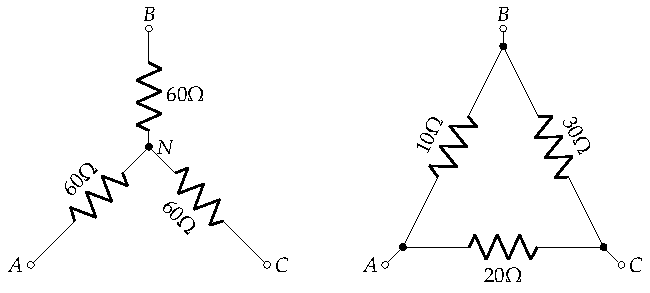
\includegraphics[height=3.5cm]{../figs/ej7_BT1.pdf}
            \caption{Ejemplo~\ref{ex.estrella-triangulo}}
            \label{fig:ejercicio7-bt1}
          \end{figure}
 	
          Se calcula primero el cambio de estrella a triángulo. Puesto
          que las tres resistencias tienen un valor de 60 $\Omega$
          ($R_a=R_b=R_c=R_Y=60\Omega$), se cumple que,
          según~\eqref{eq.triangulo-estrella-igual}:
          \begin{equation*}
            R_D=3\cdot R_Y=3\cdot 60=180\Omega
          \end{equation*}
          Puede comprobarse que se llegaría a la misma solución
          empleando las expresiones completas, donde
          $G_i=\frac{1}{R_i}=\frac{1}{60}$ S:
          \begin{align*}
            G_{ab} &= \frac{G_a \cdot G_b}{G_a + G_b + G_c}=\frac{\frac{1}{60} \cdot \frac{1}{60}}{\frac{1}{60} + \frac{1}{60} + \frac{1}{60}}=5.55\cdot 10^{-3}\,\text{S}\Rightarrow R_{ab}=\dfrac{1}{G_{ab}}=\dfrac{1}{5.55\cdot 10^{-3}}=180\Omega\\[10pt]
            G_{bc} &= \frac{G_b \cdot G_c}{G_a + G_b + G_c}=\frac{\frac{1}{60} \cdot \frac{1}{60}}{\frac{1}{60} + \frac{1}{60} + \frac{1}{60}}=5.55\cdot 10^{-3}\,\text{S}\Rightarrow R_{bc}=\dfrac{1}{G_{bc}}=\dfrac{1}{5.55\cdot 10^{-3}}=180\Omega\\[10pt]
            G_{ca} &= \frac{G_c \cdot G_a}{G_a + G_b + G_c}\frac{\frac{1}{60} \cdot \frac{1}{60}}{\frac{1}{60} + \frac{1}{60} + \frac{1}{60}}=5.55\cdot 10^{-3}\,\text{S}\Rightarrow R_{ca}=\dfrac{1}{G_{ca}}=\dfrac{1}{5.55\cdot 10^{-3}}=180\Omega
          \end{align*}

          El cambio de triángulo a estrella debe hacerse a partir de
          las ecuaciones completas, puesto que sus resistencias son
          todas diferentes:
          \begin{align*}
            R_a &= \frac{R_{ab} \cdot R_{ca}}{R_{ab} + R_{bc} + R_{ca}}=\frac{10 \cdot 20}{10 + 30 + 20}=\frac{10}{3}\Omega\\
            \\
            R_b &= \frac{R_{ab} \cdot R_{bc}}{R_{ab} + R_{bc} + R_{ca}}=\frac{10 \cdot 30}{10+30+20}=5\Omega\\
            \\
            R_c &= \frac{R_{bc} \cdot R_{ca}}{R_{ab} + R_{bc} + R_{ca}}=\frac{30 \cdot 20}{10+30+20}=10\Omega
          \end{align*}

          Los circuitos equivalentes son los mostrados en la
          Figura~\ref{fig:ejercicio7-bt1-sol}.
          \begin{figure}[H]
            \centering
            \includegraphics[height=3.5cm]{../figs/ej7_BT1_sol.pdf}%
            \caption{Ejemplo~\ref{ex.estrella-triangulo} -- Solución}
            \label{fig:ejercicio7-bt1-sol}
          \end{figure}
	    
	\end{example}
	
	\section{Aplicación de las leyes de Kirchhoff: métodos de
          análisis} \label{sec.metodos_analisis_cc} Para resolver un
        circuito, se debe conocer $U$ e $I$ en cada una de sus
        ramas. Por tanto, si se tiene un circuito formado por $r$
        ramas, el número de incógnitas será $2\cdot r$ (una de tensión
        y otra de intensidad). Por tanto, para resolver el circuito se
        deben disponer de $2\cdot r$ ecuaciones linealmente
        independientes. Para ello, basta con aplicar las leyes de
        Kirchhoff a los nudos y mallas del circuito.
	
	\begin{example}
          \label{ej.1-4}
          \textbf{Plantear el sistema de ecuaciones para resolver el
            circuito de la Figura~\ref{fig:mallas1}.}
          \begin{figure}[H]
            \centering
            \includegraphics[width=0.5\linewidth]{../figs/mallas1.pdf}
            \caption{Ejemplo~\ref{ej.1-4}}
            \label{fig:mallas1}
          \end{figure}
		
          \begin{enumerate}
          \item {Se aplica la 1LK:}
            \begin{itemize}
            \item {Nudo A:} $I_6 = I_1 + I_2$
            \item {Nudo B:} $I_1 + I_3 + I_5 = 0$
            \item {Nudo C:} $I_2 = I_3 + I_4$
            \item {Nudo D:} $I_4 = I_5 + I_6$
            \end{itemize}
            Sin embargo, se observa que no son ecuaciones linealmente
            independientes, puesto que $C=A+B+D$.
          \item {Se aplica la 2LK:}
            \begin{itemize}
            \item {Malla ABCA:}
              $I_1 \cdot R_1 - \epsilon_1 + \epsilon_2 - I_3 \cdot R_3
              - I_2 \cdot R_2 = 0$
            \item {Malla BDCB:}
              $-I_5 \cdot R_5 - I_4 \cdot R_4 + I_3 \cdot R_3 -
              \epsilon_2 = 0$
            \item {Malla ACDA:}
              $I_2 \cdot R_2 + I_4 \cdot R_4 + I_6 \cdot R_6 -
              \epsilon_3 = 0$
            \end{itemize}
          \item {Se combinan las ecuaciones:}
            \begin{align*}
              - I_1 -  I_2 + I_6  &= 0\\
              I_1 + I_3 + I_5 &= 0\\
              I_4 - I_5 - I_6 &= 0\\
              I_1 \cdot R_1 - I_2 \cdot R_2 - I_3 \cdot R_3 &= \epsilon_1 - \epsilon_2\\
              I_3 \cdot R_3 - I_4 \cdot R_4 -I_5 \cdot R_5 &= \epsilon_2\\
              I_2 \cdot R_2 + I_4 \cdot R_4 + I_6 \cdot R_6 &= \epsilon_3
            \end{align*}
          \item {Se expresan en forma matricial:}
            \begin{equation*}
              \begin{bmatrix}
                -1 & -1 & 0 & 0 & 0 & 1\\
                1 & 0 & 1 & 0 & 1 & 0\\
                0 & 0 & 0 & 1 & -1 & -1\\
                R_1 & -R_2 & - R_3 & 0 & 0 & 0\\
                0 & 0 & R_3 & - R_4 & - R_5 & 0\\
                0 & R_2 & 0 & R_4 & 0 & R_6
              \end{bmatrix} \cdot %
              \begin{bmatrix}
                I_1\\
                I_2\\
                I_3\\
                I_4\\
                I_5\\
                I_6    
              \end{bmatrix} = %
              \begin{bmatrix}
                0\\
                0\\
                0\\
                \epsilon_1 - \epsilon_2\\
                \epsilon_2\\
                \epsilon_3
              \end{bmatrix}
            \end{equation*}
          \end{enumerate}
          Se observa que es necesario resolver un sistema lineal de 6
          ecuaciones en las que las incógnitas son las corrientes de
          cada rama.
	\end{example}
	
	Esta forma de resolución de circuitos eléctricos, aunque es
        válida, no es útil por el número de ecuaciones a resolver. Por
        ello, lo más habitual es utilizar otros métodos que permiten
        la resolución de los circuitos con un número menor de
        ecuaciones. Aunque existen diferentes métodos, se van a
        presentar dos: el método de las mallas y el método de los
        nudos, explicando posteriormente una modificación de este
        último.
	
	\subsection{Método de las mallas}
        \label{sec:mallas}
	El método de las mallas simplifica el sistema de ecuaciones
        necesario mediante unas corrientes \emph{ficticias}
        denominadas \textbf{corrientes de malla}, aprovechando las
        relaciones entre tensiones de la 2LK. El procedimiento general
        de aplicación de este método es el siguiente:
	\begin{enumerate}
        \item Identificar las corrientes de rama.
        \item Asignar un sentido a las corrientes de malla, teniendo
          en cuenta que hay un total de:
          \begin{equation*} {Mallas=Ramas-Nudos+1}
          \end{equation*}
        \item Relacionar corrientes de rama con corrientes de malla.
        \item Escribir ecuaciones de mallas.
        \item Resolver la ecuación, obteniendo las corrientes de
          malla.
        \item Obtener las corrientes de rama con las relaciones del
          punto 3.
	\end{enumerate}
	
	\begin{example}
          \label{ej.1-5}
          \textbf{Plantear el sistema de ecuaciones para resolver el
            circuito de la Figura~\ref{fig:mallas1}.}
		
          Se sigue el procedimiento indicado anteriormente, donde el
          punto 1 ya está indicado en el circuito de la
          Figura~\ref{fig:mallas1}:
          \begin{enumerate}
          \item[2.] Asignar un sentido a las corrientes de malla: se
            muestra en la Figura~\ref{fig:mallas1_corrientes}
            \begin{figure}[H]
              \centering
              \includegraphics[width=0.5\linewidth]{../figs/mallas1_corrientes.pdf}
              \caption{Corrientes de malla del circuito del
                Ejemplo~\ref{ej.1-5}}
              \label{fig:mallas1_corrientes}
            \end{figure}
          \item[3.] Relacionar corrientes de rama con corrientes de
            malla:
            \begin{align*}
              I_1 &= I_a\\
              I_5 &= -I_b\\
              I_6 &= I_c\\
              I_2 &= I_c -I_a\\
              I_3 &= I_b - I_a\\
              I_4 &= I_c - I_b
            \end{align*}
          \item[4.] Escribir ecuaciones de mallas:
			
            Malla ABCA:
            $I_a \cdot R_1 - \epsilon_1 + \epsilon_2 + (I_a - I_b)
            \cdot R_3 + (I_a - I_c) \cdot R_2 = 0$
			
            Malla BDCB:
            $I_b \cdot R_5 + (I_b - I_c) \cdot R_4 + (I_b - I_a) \cdot
            R_3 - \epsilon_2 = 0$
			
            Malla ACDA:
            $(I_c - I_a) \cdot R_2 + (I_c - I_b) \cdot R_4 + I_c \cdot
            R_6 - \epsilon_3 = 0$
			
            Se reagrupan las corrientes en las ecuaciones anteriores,
            obteniéndose que:
            \begin{align*}
              I_a \cdot (R_1 + R_3 + R_2)  - I_b\cdot R_3 - I_c \cdot R_2 &= \epsilon_1 - \epsilon_2\\
              - I_a \cdot R_3 + I_b \cdot (R_5 + R_4 + R_3) - I_c \cdot R_4 &=  \epsilon_2\\
              - I_a \cdot R_2 - I_b \cdot R_4 + I_c \cdot (R_2 + R_4 + R_6) &= \epsilon_3
            \end{align*}
            que, en forma matricial:
            \begin{equation*}
              \begin{bmatrix}
                (R_1 + R_3 + R_2) &  - R_3 & - R_2 \\
                - R_3 & (R_5 + R_4 + R_3) & - R_4 \\
                - R_2 & - R_4 &  (R_2 + R_4 + R_6)
              \end{bmatrix} \cdot %
              \begin{bmatrix}
                I_a\\
                I_b\\
                I_c\\
              \end{bmatrix} = %
              \begin{bmatrix}
                \epsilon_1 - \epsilon_2\\
                \epsilon_2\\
                \epsilon_3
              \end{bmatrix}
            \end{equation*}
          \end{enumerate}
	\end{example}
	
	A partir de este ejemplo, se llega a la ecuación general que
        permite determinar el sistema de ecuaciones de un circuito de
        $n$ mallas, siendo esta:
	\begin{equation*}
          \begin{bmatrix}
            {\color{magenta}\sum R_{11}} &  {\color{teal}\pm\sum R_{12}} & {\color{teal}{\dots}} & {\color{teal}\pm\sum R_{1n}} \\
            {\color{teal}\pm\sum R_{21}} & {\color{magenta}\sum R_{22}} & {{\dots}} & {\color{teal}\pm\sum R_{2n}} \\
            {\vdots} & {\vdots} &  {\ddots} & \vdots\\
            {\color{teal}\pm\sum R_{n1}} & {\color{teal}\pm\sum R_{n2}} & \dots & {\color{magenta}\sum R_{nn}}
          \end{bmatrix} \cdot 
          \begin{bmatrix}
            I_1\\
            I_2\\
            \vdots\\
            I_n
          \end{bmatrix} = %
          \begin{bmatrix}
            {\color{orange}\sum\epsilon_1}\\
            {\color{orange}\sum\epsilon_2}\\
            {\color{orange}\vdots}\\
            {\color{orange}\sum\epsilon_n}
          \end{bmatrix}
	\end{equation*}
	donde cada {\color{magenta}$R_{ii}$} se corresponde con la
        suma de resistencias incluidas en la malla $i$; cada
        {\color{teal}$\pm R_{ij}$} se corresponde con la suma de las
        resistencias incluidas en las ramas compartidas por las mallas
        $i$ y $j$, con signo positivo ($+$) si las corrientes van en
        el mismo sentido, y negativo ($-$) en caso contrario; y cada
        {\color{orange} $\sum \epsilon_i$} es la suma algebraica de
        las fuerzas electromotrices de los generadores de la malla
        $i$, considerando un signo positivo ($+$) si contribuyen al
        giro de la corriente, y negativo ($-$) en caso contrario (es
        decir, si la corriente sale por el polo $+$ de la fuente, se
        considera positivo; si sale por el polo $-$, se considera
        negativo). Debe tenerse en cuenta que, para aplicar este
        método, \textbf{todos los generadores deben ser fuentes de
          tensión}.
	
	\begin{example}\label{ex.ejemplo_mallas}
          \textbf{Resolver el circuito del ejemplo \ref{ej.1-5} con
            los siguientes valores numéricos.}

          \begin{minipage}{0.35\linewidth}
            Datos:
            \begin{align*}
              R_1 = R_3 = R_6 &= \SI{3}{\ohm}\\
              R_2 = R_4 = R_5 &= \SI{2}{\ohm}\\
              \epsilon_1 &= \SI{245}{\volt}\\
              \epsilon_2 &= \SI{490}{\volt}\\
              \epsilon_3 &= \SI{735}{\volt}\\
            \end{align*}
          \end{minipage}
          \begin{minipage}{0.55\linewidth}
            \includegraphics{../figs/mallas1_corrientes.pdf}
          \end{minipage}

          Sustituyendo los valores numéricos en las ecuaciones
          obtenidas en el ejemplo anterior obtenemos:
          \[
            \left[\begin{array}{ccc}
                    8 & -3 & -2 \\
                    -3 & 7 & -2 \\
                    -2 & -2 & 7\\
                  \end{array}\right]%
                \cdot \left[\begin{array}{c}
                              I_a\\
                              I_b\\
                              I_c\\
                            \end{array}\right]%
                          = \left[\begin{array}{c}
                                    -245\\
                                    490\\
                                    735
                                  \end{array}\right]
                              \]
                              cuya solución es:

\begin{align*}
  I_a &= \SI{65}{\ampere}\\
  I_b &= \SI{145}{\ampere}\\
  I_c &= \SI{165}{\ampere}
\end{align*}

Por tanto, los valores de las corrientes de rama son:

\begin{align*}
  I_1 &= \SI{65}{\ampere}\\
  I_2 &= \SI{100}{\ampere}\\
  I_3 &= \SI{80}{\ampere}\\
  I_4 &= \SI{20}{\ampere}\\
  I_5 &= \SI{-145}{\ampere}\\
  I_6 &= \SI{165}{\ampere}
\end{align*}
\end{example}
	
	\begin{remark}
          El Ejemplo~\ref{ex.mallas_dependiente} incluye contenido
          avanzado que queda fuera del alcance de la asignatura.
	\end{remark}
	
	\begin{example}\label{ex.mallas_dependiente}
          \textbf{Calcular la corriente $I$ en el circuito de la
            Figura~\ref{fig:ejemplo_mallas_dependiente}.}
          \begin{figure}[H]
            \centering
            \includegraphics[width=0.35\linewidth]{../figs/ejemplo_mallas_dependiente.pdf}
            \caption{Ejemplo~\ref{ex.mallas_dependiente}}
            \label{fig:ejemplo_mallas_dependiente}
          \end{figure}
	    
          En este caso, no se puede transformar el generador de
          intensidad en uno de tensión, por lo que se le asigna una
          caída de tensión arbitraria (y desconocida), $U_{g1}$,
          considerándolo como un generador de tensión. Posteriormente,
          al plantear el sistema de ecuaciones, se añadirá una
          ecuación adicional, puesto que la intensidad de esa rama es
          conocida (2 A). El circuito queda como se muestra en la
          Figura~\ref{fig:mallas_dpendiente_sol}.
          \begin{figure}[H]
            \centering
            \includegraphics[width=0.35\linewidth]{../figs/ejemplo_mallas_dependiente_sol.pdf}
            \caption{Ejemplo~\ref{ex.mallas_dependiente} -- Mallas}
            \label{fig:mallas_dpendiente_sol}
          \end{figure}
	    
          Se plantea el método de mallas en forma matricial:
          \begin{equation*}
            \begin{bmatrix}
              5 & -2 \\
              -2 & 7 
            \end{bmatrix} \cdot 
            \begin{bmatrix}
              I_a\\
              I_b
            \end{bmatrix} = %
            \begin{bmatrix}
              -4-U_{g1} \\
              4-3\cdot U_r
            \end{bmatrix}
          \end{equation*}
          donde se sabe que $I_a=-2$ A. Además, la tensión $U_r$ se
          puede expresar, a partir d ela ley de Ohm y las relaciones
          entre las corrientes de malla como:
          \begin{equation*}
	    U_r=(I_a-I_b)\cdot R_{2\Omega}=(I_a-I_b)\cdot 2 = (-2-I_b)\cdot 2=-4-2\, I_b
          \end{equation*}
          Reemplazando en la segunda ecuación del sistema:
          \begin{equation*}
	    -2\, I_a+7\,I_b=4-3\,U_r; -2\,(-2)+7\, I_b=4-3\,(-4-2\,I_b); 4+7\,I_b=4+12+6\,I_b\Rightarrow I_b=12\, A 
          \end{equation*}
          Por lo que $I=-I_b=-12$ A
	\end{example}
	

	
	\subsection{Método de los nudos}
        \label{sec:nudos}
	El método de los nudos es otro de los procedimientos de
        análisis utilizados en teoría de circuitos, aprovechando las
        relaciones entre corrientes de la 1LK. El procedimiento
        general de aplicación de este método es el siguiente:
	\begin{enumerate}
        \item Identificar las corrientes de rama.
        \item Identificar los nudos independientes, que son:
          \begin{equation*} {Nudos\;\;Independientes=Nudos-1}
          \end{equation*}
        \item Aplicar la 1LK a cada nudo independiente.
        \item Determinar las tensiones en los receptores a partir de
          la Ley de Ohm (considerando la resistencia y, después, la
          conductancia).
        \item Combinar las ecuaciones de los puntos 3 y 4.
        \item Resolver la ecuación.
	\end{enumerate}
	
	\begin{example}\label{ej.1-6}
          \textbf{Plantear el sistema de ecuaciones para resolver el
            circuito de la Figura~\ref{fig:nudos}.}
          \begin{figure}[H]
            \centering \includegraphics{../figs/nudos.pdf}
            \caption{Ejemplo~\ref{ej.1-6}}
            \label{fig:nudos}
          \end{figure}
		
          Se sigue el procedimiento indicado anteriormente, llegando
          únicamente hasta el punto 5:
		
          \begin{enumerate}
          \item Identificar las corrientes de rama: identificadas en
            la Figura~\ref{fig:nudos}
          \item Identificar los nudos independientes, que son $A$ y
            $B$ en la Figura~\ref{fig:nudos}.
          \item Aplicar la 1LK a cada nudo independiente:
			
            Nudo A
            \begin{equation*}
              I_{g1} - I_a - I_{ab} = 0
            \end{equation*}
			
            Nudo B
            \begin{equation*}
              I_{ab} - I_{g2} - I_b = 0
            \end{equation*}
          \item Determinar las tensiones en los receptores a partir de
            la Ley de Ohm (considerando la resistencia y, después, la
            conductancia):
            \begin{align*}
              U_A = U_{R_1} &= I_a \cdot R_1\rightarrow I_a=U_A\cdot G_1\\
              U_B = U_{R_3} &= I_b \cdot R_3\rightarrow I_b=U_B\cdot G_3\\
              U_{AB}=U_{R_2} &= I_{ab} \cdot R_2\rightarrow I_{ab}=(U_A-U_B)\cdot G_2\\
            \end{align*}
          \item Combinar las ecuaciones de los puntos 3 y 4:
			
            Nudo A
            \begin{equation*}
              I_{g1} - U_A \cdot G_1 - (U_A - U_B) \cdot G_2 = 0\rightarrow I_{g1} = U_A \cdot (G_1 + G_2) - U_B \cdot G_2 
            \end{equation*}
			
            Nudo B
            \begin{equation*}
              (U_A - U_B) \cdot G_2 - I_{g2} - U_B \cdot G_3 = 0 \rightarrow  - I_{g2} = - U_A \cdot G_2 + U_B \cdot (G_2 + G_3)
            \end{equation*}
			
            Estas ecuaciones se pueden expresar en forma matricial de
            la siguiente manera:
            \begin{equation*}
              \begin{bmatrix}
                G_1 + G_2 & - G_2\\
                -G_2 & G_2 + G_3
              \end{bmatrix} \cdot%
              \begin{bmatrix}
                U_A\\
                U_B
              \end{bmatrix} = %
              \begin{bmatrix}
                I_{g1}\\
                -I_{g2}
              \end{bmatrix}
            \end{equation*}
          \end{enumerate}
	\end{example}
	
	A partir de este ejemplo, se llega a la ecuación general que
        permite determinar el sistema de ecuaciones de un circuito de
        $n$ nudos, siendo esta:
	\begin{equation*}
          \begin{bmatrix}
            {\color{magenta}\sum G_{1}} &  {\color{teal}-\sum G_{12}} & {\color{teal}{\dots}} & {\color{teal}-\sum G_{1n}} \\
            {\color{teal}-\sum G_{21}} & {\color{magenta}\sum G_{2}} & {{\dots}} & {\color{teal}-\sum G_{2n}} \\
            {\vdots} & {\vdots} &  {\ddots} & \vdots\\
            {\color{teal}-\sum G_{n1}} & {\color{teal}-\sum G_{n2}} & \dots & {\color{magenta}\sum G_{n}}
          \end{bmatrix} \cdot 
          \begin{bmatrix}
            U_1\\
            U_2\\
            \vdots\\
            U_n
          \end{bmatrix} = %
          \begin{bmatrix}
            {\color{orange}\sum I_{g1}}\\
            {\color{orange}\sum I_{g2}}\\
            {\color{orange}\vdots}\\
            {\color{orange}\sum I_{gn}}
          \end{bmatrix}
	\end{equation*}
	donde cada {\color{magenta}$G_{i}$} se corresponde con la suma
        de conductancias conectadas al nudo $i$; cada
        {\color{teal}$ G_{ij}$} se corresponde con la suma de las
        conductancias conectadas entre los nudos $i$ y $j$; y cada
        {\color{orange} $\sum I_{gi}$} es la suma algebraica de las
        corrientes de los generadores conectados al nudo $i$,
        considerando un signo positivo ($+$) si el generador inyecta
        corriente en el nudo, y negativo ($-$) en caso contrario. Debe
        tenerse en cuenta que para aplicar este método \textbf{todos
          los generadores deben ser fuentes de corriente}.
	
	\begin{example}\label{ex.nudos}
          \textbf{En el circuito de la Figura~\ref{fig:nudos_fuentes},
            se debe emplear el método de los nudos para determinar:
            \begin{itemize}
            \item Las tensiones en los nudos A y B
            \item Las corrientes de rama señaladas
            \item El balance de potencias, diferenciando entre
              elementos activos y elementos pasivos
            \end{itemize}
            Datos:
            $\epsilon_1=\qty{6}{\volt};\;
            \epsilon_2=\qty{12}{\volt};\;
            \epsilon_3=\qty{24}{\volt};\; I_{g1}= \qty{15}{\ampere};\;
            I_{g2} = \qty{9}{\ampere};\; I_{g3}= \qty{6}{\ampere};\;
            R_{1}= R_3 = R_4 = R_5 = \qty{2}{\ohm};\; R_{2}=
            \qty{1}{\ohm}$}
          \begin{figure}[H]
            \centering \includegraphics{../figs/nudos_fuentes.pdf}
            \caption{Ejemplo~\ref{ex.nudos}}
            \label{fig:nudos_fuentes}
          \end{figure}

          En el circuito hay tres fuentes de tensión en serie con
          resistencias, que se deben transformar en fuentes de
          corriente para poder aplicar el método de nudos:

          \begin{figure}[H]
            \centering
            \includegraphics[scale=0.9]{../figs/nudos_fuentes2.pdf}
          \end{figure}

          \vspace{-3mm}
          \begin{align*}
            I_{\epsilon,1}&=\dfrac{\epsilon_1}{R_1}=\dfrac{6}{2}=\qty{3}{\ampere}\\
            I_{\epsilon,2}&=\dfrac{\epsilon_2}{R_2}=\dfrac{12}{1}=\qty{12}{\ampere}\\
            I_{\epsilon,3}&=\dfrac{\epsilon_3}{R_3}=\dfrac{24}{2}=\qty{12}{\ampere}
          \end{align*}

          \vspace{2mm} Aplicamos ahora la ecuación general de método
          de los nudos al circuito, que consta únicamente de 2 nudos
          independientes:
          \begin{equation*}
            \begin{bmatrix}
              \dfrac{1}{2}+\dfrac{1}{2}+\dfrac{1}{1} & -\dfrac{1}{1}\\[10pt]
              -\dfrac{1}{1} & \dfrac{1}{1}+\dfrac{1}{2}+\dfrac{1}{2}
            \end{bmatrix}
            \cdot
            \begin{bmatrix}
              \vphantom{\dfrac{1}{1}} U_A\\[10pt]
              \vphantom{\dfrac{1}{1}} U_B
            \end{bmatrix}
            =
            \begin{bmatrix}
              \vphantom{\dfrac{1}{1}} 3+12-15-6\\[10pt]
              \vphantom{\dfrac{1}{1}} 15+9+12-12
            \end{bmatrix}
          \end{equation*}
    
          \vspace{5mm} Cuya solución es:

          \vspace{-5mm}
          \begin{align*}
            U_A&=\qty{4}{\volt}\\
            U_B&=\qty{14}{\volt}
          \end{align*}

          A partir de las tensiones, se determinan las corrientes de
          rama señaladas, aplicando 2LK:

          % \begin{align*}
          %   V_A &= E_1 - I_{R1} R_1 = I_{R4} \cdot R_4\\
          %   V_{AB} &= E_2 - I_{R2} R_2\\
          %   V_B &= E_3 - I_{R3} R_3 = I_{R5} \cdot R_5\\
          % \end{align*}

          \vspace{-5mm}
          \begin{align*}
            U_A=\epsilon_1-I_{R1}\,R_1 \quad &\Rightarrow \quad {I_{R1}=\dfrac{6-4}{2}= \qty{1}{\ampere}}\\
            U_{AB}=U_A-U_B=-10=\epsilon_2 - I_{R2}\, R_2 \quad &\Rightarrow \quad I_{R2} = \dfrac{12-(-10)}{1}= \qty{22}{\ampere}\\
            U_B=\epsilon_3-I_{R3}\,R_3 \quad &\Rightarrow \quad I_{R3}=\dfrac{24-14}{2}= \qty{5}{\ampere}\\
            I_{R4}=\dfrac{U_A}{R_4}&=\dfrac{4}{2}= \qty{2}{\ampere}\\
            I_{R5}=\dfrac{U_B}{R_5}&=\dfrac{14}{2}= \qty{7}{\ampere}
          \end{align*}

          \vspace{2mm} Se recomienda comprobar que estos resultados
          cumplen la 1LK en cada uno de los 2 nudos independientes del
          \underline{circuito original} (antes de transformar las
          fuentes de tensión, porque tambien podríais haber cometido
          errores al transformar las fuentes), para asegurarse de que
          la resolución es correcta.

          \vspace{4mm} Ya tenemos toda la información necesaria para
          formular el balance de potencias pedido en el último
          apartado:

          \begin{itemize}
          \item \textbf{Potencia de los generadores:}
            \begin{align*}
              P_{Ig1} &= I_1 U_{BA} = \qty{150}{\watt}\\
              P_{Ig2} &= I_2 V_{B} = \qty{126}{\watt}\\
              P_{Ig3} &= I_3 (-V_{A}) = - \qty{24}{\watt}\\
              P_{\epsilon_1} &= \epsilon_1 I_{R1} = \qty{6}{\watt}\\
              P_{\epsilon_2} &= \epsilon_2 I_{R2} = \qty{264}{\watt}\\
              P_{\epsilon_3} &= \epsilon_3 I_{R3} = \qty{120}{\watt}
            \end{align*}
            Los elementos activos aportan un total de
            \qty{642}{\watt}.
          \item \textbf{Potencia de las resistencias:}
            \begin{align*}
              P_{R1} &= (I_{R1})^2 R_1 = \qty{2}{\watt}\\
              P_{R2} &= (I_{R2})^2 R_2 = \qty{484}{\watt}\\
              P_{R3} &= (I_{R3})^2 R_3 = \qty{50}{\watt}\\
              P_{R4} &= (I_{R4})^2 R_4 = \qty{8}{\watt}\\
              P_{R5} &= (I_{R5})^2 R_5 = \qty{98}{\watt}
            \end{align*}
            Las resistencias disipan un total de \SI{642}{\watt}.
          \end{itemize}

          Comprobamos que la potencia total entregada por los
          generadores es igual a la potencia total consumida por las
          resistencias.

        \end{example}
	
        \subsubsection{\textsuperscript{TC2} Método de los nudos
          modificados}\label{sec.nudos_modificados}
	
	Otra manera de plantear el método de los nudos es mediante el
        conocido como método de los nudos modificados, que permite que
        en el circuito haya \textbf{fuentes de tensión y de
          corriente}. En este caso, tras elegir el nudo de referencia
        ($U_{ref}=0$), se aplica la 1LK a cada uno de los nudos
        independientes ($N-1$) del siguiente modo:
	\begin{enumerate}
        \item Se supone que, en cada nudo independiente, las
          corrientes \textbf{salen} de él
        \item Cada nudo debe cumplir con la 1LK: $\sum I=0$
        \item En cada nudo, aplicar la siguiente expresión:
          \begin{equation*}
            I_{i,j}=\dfrac{U_i-U_j+\sum\pm \epsilon_g}{\sum R}
          \end{equation*}
          siendo $I_{i,j}$ la corriente que va del nudo $i$ al $j$,
          $U_i$ la tensión del nudo del que se sale, $U_j$ la tensión
          del nudo al que se llega, $\epsilon_g$ son las $fem$ de los
          generadores, considerando el signo $+$ si la corriente de la
          rama sale por el polo positivo y el signo $-$ si la
          corriente sale por el negativo.
	\end{enumerate}
	
	\begin{example}\label{ex.nudos_modificados}
          \textbf{Determinar las tensiones en los nudos A y B en el
            circuito de la Figura~\ref{fig:nudos_fuentes}.}
	    
          Se trabaja con el circuito original.
	    
          \textbf{Nudo A}
          \begin{align*}
            I_{R1}& + I_{R2} + I_{R4} + I_{g1} + I_{g3} = 0\\
            I_{R1}&=\dfrac{U_A-0-\epsilon_1}{R_1}=\dfrac{U_A-6}{2}\\
            I_{R2}&=\dfrac{U_A-U_B-\epsilon_2}{R_2}=\dfrac{U_A-U_B-12}{1}\\
            I_{R4}&=\dfrac{U_A-0}{R_4}=\dfrac{U_A}{2}\\
            I_{g1}&=15\,A\\
            I_{g3}&=6\,A
          \end{align*}
	    
          \textbf{Nudo B}
          \begin{align*}
            I_{R2}& + I_{R3} + I_{R5} + I_{g1} + I_{g2} = 0\\
            I_{R2}&=\dfrac{U_B-U_A+\epsilon_2}{R_2}=\dfrac{U_B-U_A+12}{1}\\
            I_{R3}&=\dfrac{U_B-0-\epsilon_3}{R_3}=\dfrac{U_B-24}{2}\\
            I_{R5}&=\dfrac{U_B-0}{R_5}=\dfrac{U_B}{2}\\
            I_{g1}&=-15\,A\\
            I_{g2}&=-9\,A
          \end{align*}
	    
          Combinando las ecuaciones del nudo A, se obtiene que:
          \begin{equation*}
            \dfrac{U_A-6}{2}+\dfrac{U_A-U_B-12}{1}+\dfrac{U_A}{2}+15+6=0\Rightarrow 2\,U_A-U_B=-6
          \end{equation*}
          De manera análoga, con el nudo B:
          \begin{equation*}
            \dfrac{U_B-U_A+6}{1}+\dfrac{U_B-24}{2}+\dfrac{U_B}{2}-15-6=0\Rightarrow -U_A+2\,U_B=24
          \end{equation*}
          Resolviendo el sistema de ecuaciones, se llega a la
          conclusión de que:
          \begin{align*}
            U_A&=4\,V\\
            U_B&=14\,V
          \end{align*}

	\end{example}
	
	\begin{example}\label{ex.nudos_mod_fdep}
          \textbf{Calcular la corriente $I$ en el circuito de la
            Figura~\ref{fig:ejemplo_mallas_dependiente}.}
	    
          Se considera como referencia (masa) el nudo de abajo. La 1LK
          aplicada al nudo de arriba queda:
          \begin{equation*}
            2+\dfrac{U_A-0-4}{2}+\dfrac{U_A-0-3\,U_r}{5}=2+\dfrac{U_A-4}{2}+\dfrac{U_A-3\,U_r}{5}
          \end{equation*}
          Además, el valor de $U_r$ se puede obtener a partir de la
          ley de Ohm:
          \begin{equation*}
            U_r=2\, I_{R_2}=2\cdot \left( \dfrac{U_A-4}{2} \right)=U_A-4
          \end{equation*}
          Y, reemplazando este valor en la ecuación de la 1LK se
          obtiene que:
          \begin{equation*}
            2+\dfrac{U_A-4}{2}+\dfrac{U_A-3\,U_A+12}{5}=0\Rightarrow U_A=-24\,V
          \end{equation*}
          por lo que $I$:
          \begin{equation*}
            I=-\left(\dfrac{U_A-3\,U_r}{5} \right)=-\left(\dfrac{24-3\,(-24-4)}{5}\right)=-12\,A
          \end{equation*}
	\end{example}

        \subsection{\textsuperscript{TC2} Movilidad de fuentes}
        \label{sec:movilidad-fuentes}

        En el desarrollo del método de las mallas (apartado \ref{sec:mallas}) se observó que las fuentes de corriente debían ser sustituidas por fuentes de tensión equivalente. Asimismo, en el método de los nudos (apartado \ref{sec:nudos}) las fuentes de tensión deben ser reemplazadas por fuentes de corriente equivalentes. Ahora bien, estas transformaciones son posibles cuando se trata de fuentes reales. En el caso de fuentes ideales, es necesario aplicar un enfoque diferente. Una solución posible es la modificación de la geometría del circuito mediante la movilidad de fuentes.

        \subsubsection{Movilidad de fuentes de tensión}
\label{sec:movilidad-fuentes-tension}

La figura \ref{fig:movilidad-fuente-tension} representa una parte de un circuito que contiene una fuente ideal de tensión conectada entre dos nudos. La figura \ref{fig:movilidad-fuente-tension1} es una modificación de la geometría de este circuito en el que la fuente se ha desdoblado en dos y ha cambiado su posición a la parte superior. Es inmediato comprobar que los cuatro elementos pasivos conectados en los nudos están sometidos a las mismas tensiones en los dos circuitos. Por otra parte, dado que las dos fuentes son del mismo valor y están conectadas al mismo nudo en su parte inferior, su terminal superior está al mismo potencial. Por tanto, están conectadas en paralelo y pueden simplificarse por una única fuente de tensión, lo que nos lleva de vuelta al circuito original. Un circuito alternativo se representa en la figura \ref{fig:movilidad-fuente-tension2}, en el que el desdoblamiento de fuentes se ha trasladado al nudo inferior. 

Al aplicar esta movilidad, se obtienen fuentes reales de tensión que, a su vez, pueden ser transformadas en fuentes de corriente equivalentes. 
\begin{figure}[H]
  \centering
  \subfloat[Circuito original]{\includegraphics[height=4cm]{../figs/ModificacionGeometria_FuenteTension.pdf}\label{fig:movilidad-fuente-tension}}\hfill
  \subfloat[Circuito modificado (1)]{\includegraphics[height=4cm]{../figs/ModificacionGeometria_FuenteTension2.pdf}\label{fig:movilidad-fuente-tension1}}\hfill
  \subfloat[Circuito modificado (2)]{\includegraphics[height=4cm]{../figs/ModificacionGeometria_FuenteTension3.pdf}\label{fig:movilidad-fuente-tension2}}
  \caption{Modificación de la geometría de un circuito con la movilidad de una fuente de tensión.}
\end{figure}
        \subsubsection{Movilidad de fuentes de corriente}
\label{sec:movilidad-fuentes-corriente}

La figura \ref{fig:movilidad-fuente-corriente} representa una parte de un circuito que contiene una fuente ideal de corriente conectada entre dos nudos. La figura \ref{fig:movilidad-fuente-corriente1} es una modificación de la geometría de este circuito en el que la fuente ha desaparecido de su ubicación original y se ha replicado tres veces, una por elemento pasivo. Se puede comprobar que el balance de corrientes de cada uno es el mismo en los dos circuitos por lo que, a pesar de esta modificación de la geometría, se trata de circuitos equivalentes.

Al aplicar esta movilidad, se obtienen fuentes reales de corriente que, a su vez, pueden ser transformadas en fuentes de tensión equivalentes. 

\begin{figure}[H]
  \centering
  \subfloat[Circuito original]{\includegraphics[height=4cm]{../figs/ModificacionGeometria_FuenteCorriente.pdf}\label{fig:movilidad-fuente-corriente}}\hfill
  \subfloat[Circuito modificado]{\includegraphics[height=4cm]{../figs/ModificacionGeometria_FuenteCorriente2.pdf}\label{fig:movilidad-fuente-corriente1}}
  \caption{Modificación de la geometría de un circuito con la movilidad de una fuente de corriente.}
\end{figure}



%%% Local Variables:
%%% mode: latex
%%% TeX-master: "TC"
%%% ispell-local-dictionary: "castellano"
%%% End:
